\chapter{Numerical Solution of Ordinary Differential Equations}

\section{Ordinary Differential Equations: Initial Value Problems (ODE-IVPs)}

Many physical processes that we model in engineering and science are dynamic. This means that first-principles models describing these processes can be formulated as differential equations, which describe how system variables change with respect to time or space. We can express a general dynamic model as a system of first-order ordinary differential equations (ODEs):
\begin{equation}
    \frac{d\mathbf{x}(t)}{dt} = \mathbf{f}(\mathbf{x}(t), \mathbf{u}(t), t; \boldsymbol{\theta})
\end{equation}
This system is coupled with an initial condition, which specifies the state of the system at a starting time $t_0$:
\begin{equation}
    \mathbf{x}(t_0) = \mathbf{x}_0
\end{equation}
Here, $\mathbf{x}(t)$ is the state vector, which contains the set of dynamic variables we want to solve for; $t$ is time; $\mathbf{u}(t)$ is a vector of time-dependent inputs that we specify (e.g., an external force), which is sometimes considered part of $\mathbf{f}$; $\boldsymbol{\theta}$ is a vector of time-independent parameters (e.g., mass, reaction constants); and $\mathbf{x}_0$ is the vector of initial values for the state variables at time $t_0$.

Usually, we are interested in finding the solution (the values of the state vector $\mathbf{x}(t)$) within some time domain, $t \in [t_0, t_f]$. This task is formally known as the \textbf{initial value problem (IVP)}. For simplicity, we will often group the inputs $\mathbf{u}(t)$ and parameters $\boldsymbol{\theta}$ into the function $\mathbf{f}$ and write the IVP more compactly:
\begin{equation}
    \frac{d\mathbf{x}(t)}{dt} = \mathbf{f}(\mathbf{x}(t), t) \quad \forall t \in [t_0, t_f], \text{ given } \mathbf{x}(t_0) = \mathbf{x}_0
    \label{eq:ode-ivp}
\end{equation}
By convention, the initial time $t_0$ is often set to zero.

\begin{exampleBox}
    \textbf{Example: Consecutive Reaction System}
    
    Consider a series of first-order reactions $A \xrightarrow{k_1} B \xrightarrow{k_2} C$ in a batch reactor. Define the state vector as $\mathbf{x}(t) = [C_A(t), C_B(t), C_C(t)]^\top$, where $C_i$ represents the concentration of species $i$. The system is described by
    \begin{equation}
    \frac{d\mathbf{x}}{dt} = \begin{bmatrix} \dot{C}_A \\ \dot{C}_B \\ \dot{C}_C \end{bmatrix} = \begin{bmatrix} -k_1 C_A \\ k_1 C_A - k_2 C_B \\ k_2 C_B \end{bmatrix}
    \end{equation}
    with rate constants $\boldsymbol{\theta} = [k_1, k_2]^\top$ and initial concentrations $\mathbf{x}_0 = [C_{A,0}, C_{B,0}, C_{C,0}]^\top$ at $t_0 = 0$.
\end{exampleBox}

The challenge comes from the function $\mathbf{f}(\mathbf{x}(t), t)$. Since $\mathbf{f}$ can be an arbitrary nonlinear function of the state vector, a closed-form, analytical solution for $\mathbf{x}(t)$ rarely exists. We must therefore turn to numerical methods. The goal of a numerical method is to solve this equation by finding the state vector $\mathbf{x}$ at a finite number of discrete points within the time domain $[t_0, t_f]$. When developing and choosing these methods, we will need to characterize two important properties: the \textbf{accuracy} (how close our numerical solution is to the true, unknown solution) and the \textbf{stability} (whether errors grow uncontrollably) of the solution methods.

\subsection{Rewriting Higher-Order ODEs}
The numerical methods we will study are designed for systems of \textit{first-order} ODEs. Fortunately, any higher-order differential equation can be rewritten as a system of first-order equations by introducing new variables for the derivatives. The procedure is very straightforward: for an $n$th-order ODE, define $n$ new state variables where each represents a successive derivative of the original variable. For a second-order equation in $x(t)$, we define:
\begin{align}
    x_1 &= x \\
    x_2 &= \frac{dx}{dt}
\end{align}
Then the $n$th derivative becomes a first-order equation: $dx_n/dt = $ (expression from the original ODE).

\begin{exampleBox}
\textbf{Example: Driven Mass-Spring-Damper}

The second-order equation $m\ddot{x} + b\dot{x} + kx = f(t)$ (dots are time derivatives, a common notation in physics/engineering) can be rewritten by defining the state vector $\mathbf{x}(t) = [x(t), v(t)]^\top$ where $v = \dot{x}$. This gives the first-order system:
\begin{equation}
    \frac{d\mathbf{x}}{dt} = {\renewcommand{\arraystretch}{2}
    \begin{bmatrix} \dfrac{dx}{dt} \\ \dfrac{dv}{dt} \end{bmatrix} = \begin{bmatrix} v \\ \dfrac{f(t) - bv - kx}{m} \end{bmatrix}}
\end{equation}
with initial condition $\mathbf{x}_0 = [x(t_0), v(t_0)]^\top$.
\end{exampleBox}

This pattern generalizes to ODEs of any order: simply add new state variables for each derivative up to order $n-1$.

\subsection{Local Truncation Error}
To understand the accuracy of a method, we must first estimate the local truncation error (LTE). This is the error we introduce in a single step, assuming that the solution we start with at $t_i$, $\mathbf{x}(t_i)$, is perfectly accurate (i.e., $\mathbf{x}(t_i) = \mathbf{x}_{\text{exact}}(t_i)$). We can find the exact value of the solution at $t_{i+1}$ by using a Taylor expansion of $\mathbf{x}_{\text{exact}}(t)$ around the point $t_i$:
\begin{equation}
    \mathbf{x}_{\text{exact}}(t_{i+1}) = \mathbf{x}_{\text{exact}}(t_i) + \sum_{j=1}^{\infty} \frac{1}{j!} (\Delta t_i)^j \frac{d^j \mathbf{x}}{dt^j} \bigg|_{t_i}
\end{equation}
Our numerical method provides an approximation $\mathbf{x}(t_{i+1})$. The local truncation error is the difference between this exact value and our approximation.

\begin{definitionBox}
The \textbf{local truncation error}, $\epsilon$, is defined as the magnitude (norm) of the difference between the exact solution at $t_{i+1}$ and the numerical approximation at $t_{i+1}$, assuming the numerical solution was exact at $t_i$:
\begin{equation}
\epsilon = \| \mathbf{x}_{\text{exact}}(t_{i+1}) - \mathbf{x}(t_{i+1}) \|
\end{equation}
\end{definitionBox}

We typically characterize this error using big-O notation to describe how it scales with the step size $\Delta t_i$. We say the local truncation error is of order $p$, or $O(\Delta t_i^p)$, if the following limit exists for some constant $C > 0$:
\begin{equation}
\lim_{\Delta t_i \to 0^+} \frac{\| \mathbf{x}_{\text{exact}}(t_{i+1}) - \mathbf{x}(t_{i+1}) \|}{(\Delta t_i)^p} = C
\end{equation}
A method with LTE of $O(\Delta t_i^p)$ is said to be $(p-1)$-th order accurate.

\section{Explicit Methods for Solving ODE-IVPs}
Numerical methods for IVPs work by stepping forward in time. We start at $t_i$ with a known solution $\mathbf{x}(t_i)$ and try to approximate the solution at a future point in time, $t_{i+1}$. An \textbf{explicit method} calculates the future state $\mathbf{x}(t_{i+1})$ using only information from the current (or previous) time steps. The general form for a one-step explicit method is:
\begin{equation}
    \mathbf{x}(t_{i+1}) = \mathbf{x}(t_i) + \Delta t_i \mathbf{g}(\mathbf{x}(t_i), t_i, \Delta t_i)
\end{equation}
Here, $\Delta t_i = t_{i+1} - t_i$ is the step size, which controls the local truncation error in the solution. The function $\mathbf{g}(\mathbf{x}(t_i), t_i, \Delta t_i)$ is the workhorse of the method. It is designed to be a good approximation of the change in $\mathbf{x}$ over the step. It has the goal of minimizing the error at a given $\Delta t_i$ while also maintaining numerical stability.

\subsection{The Explicit (Forward) Euler Method}

The simplest explicit method is the explicit Euler (also known as forward Euler) method. It is defined by the formula
\begin{equation}
\mathbf{x}(t_{i+1}) = \mathbf{x}(t_i) + \Delta t_i \mathbf{f}(\mathbf{x}(t_i), t_i)
\end{equation}
This is an instance of our general explicit form where the function $\mathbf{g}$ is simply $\mathbf{g}(\mathbf{x}(t_i), t_i, \Delta t_i) = \mathbf{f}(\mathbf{x}(t_i), t_i)$. This method can be derived directly from a forward finite difference approximation for the derivative $\mathbf{x}'(t)$ at time $t_i$:
\begin{equation}
    \frac{d\mathbf{x}}{dt} \bigg|_{t_i} \approx \frac{\mathbf{x}(t_{i+1}) - \mathbf{x}(t_i)}{\Delta t_i}
\end{equation}
Since we know that $\frac{d\mathbf{x}}{dt} = \mathbf{f}(\mathbf{x}, t)$ (this is the definition of the function $\mathbf{f}$ as per \autoref{eq:ode-ivp}), we can set them equal:
\begin{equation}
    \mathbf{f}(\mathbf{x}(t_i), t_i) \approx \frac{\mathbf{x}(t_{i+1}) - \mathbf{x}(t_i)}{\Delta t_i}
\end{equation}
Rearranging for $\mathbf{x}(t_{i+1})$ gives the forward Euler formula. Visually, this method can be understood by looking at the integral form of the ODE. The exact solution is:
\begin{equation}
    \mathbf{x}(t_{i+1}) = \mathbf{x}(t_i) + \int_{t_i}^{t_{i+1}} \mathbf{f}(\mathbf{x}(t'), t') dt'
\end{equation}
The forward Euler method approximates this integral by assuming the integrand, $\mathbf{f}(\mathbf{x}(t'), t')$, is constant over the entire interval $[t_i, t_{i+1}]$ and is equal to its value at the start of the interval, $\mathbf{f}(\mathbf{x}(t_i), t_i)$. This is the simplest rectangular approximation (a zero-order hold) of the integral. The method, therefore, takes a step from $\mathbf{x}(t_i)$ by moving in the direction of the tangent $\mathbf{f}(\mathbf{x}(t_i), t_i)$ for a duration of $\Delta t_i$.


\begin{figure}[H]
    \centering
    \includegraphics[width=0.8\textwidth]{figs/ode/forward_euler_demo.pdf}
    \caption{Forward (explicit) Euler visualization. The exact solution $\mathbf{x}(t)$ (black) is compared with the forward Euler approximation (red) using step $h=\Delta t$. At each grid point $t_i$, the method advances via $\mathbf{x}_{i+1}=\mathbf{x}_i+\Delta t\,\mathbf{f}(\mathbf{x}_i,t_i)$ using the slope at the left endpoint.}

    \label{fig:forward_euler_demo}
\end{figure}


\paragraph*{Local Error of Euler's Method}

Let's estimate the local truncation error for this method. We again start with the Taylor expansion of the exact solution:
\begin{equation}
    \mathbf{x}_{\text{exact}}(t_{i+1}) = \mathbf{x}_{\text{exact}}(t_i) + \Delta t_i \frac{d\mathbf{x}}{dt}\bigg|_{t_i} + \frac{1}{2}(\Delta t_i)^2 \frac{d^2\mathbf{x}}{dt^2}\bigg|_{t_i} + O(\Delta t_i^3)
\end{equation}
By our problem definition, $\frac{d\mathbf{x}}{dt} = \mathbf{f}(\mathbf{x}, t)$. Assuming $\mathbf{x}(t_i) = \mathbf{x}_{\text{exact}}(t_i)$, we have
\begin{equation}
    \frac{d\mathbf{x}}{dt}\bigg|_{t_i} = \mathbf{f}(\mathbf{x}_{\text{exact}}(t_i), t_i) = \mathbf{f}(\mathbf{x}(t_i), t_i)
\end{equation}
Substituting this into the expansion gives
\begin{equation}
    \mathbf{x}_{\text{exact}}(t_{i+1}) = \underbrace{\mathbf{x}(t_i) + \Delta t_i \mathbf{f}(\mathbf{x}(t_i), t_i)}_{\text{forward Euler approx. } \mathbf{x}(t_{i+1})} + \frac{1}{2}(\Delta t_i)^2 \frac{d^2\mathbf{x}}{dt^2}\bigg|_{t_i} + O(\Delta t_i^3)
\end{equation}
The first two terms are precisely the forward Euler approximation $\mathbf{x}(t_{i+1})$. The local truncation error $\epsilon$ is therefore the remainder:
\begin{equation}
    \epsilon = \| \mathbf{x}_{\text{exact}}(t_{i+1}) - \mathbf{x}(t_{i+1}) \| = \left\| \frac{1}{2}(\Delta t_i)^2 \frac{d^2\mathbf{x}}{dt^2}\bigg|_{t_i} + O(\Delta t_i^3) \right\|
\end{equation}
Thus, the local truncation error is $O(\Delta t_i^2)$. As $\Delta t_i \to 0$, the ratio $\epsilon / (\Delta t_i)^2$ approaches a constant $C > 0$. This is the error from just one step. What about the global error? Over many iterations of this method, how bad does our solution become?

\paragraph*{Global Error of Euler's Method} Let's assume a constant step size $\Delta t$. At each step, we introduce a local error of $O(\Delta t^2)$.
\begin{align}
    \mathbf{x}(t_1) &= \mathbf{x}(t_0) + \Delta t \mathbf{f}(\mathbf{x}_0, t_0) = \mathbf{x}_{\text{exact}}(t_1) + O(\Delta t^2) \\
    \mathbf{x}(t_2) &= \mathbf{x}(t_1) + \Delta t \mathbf{f}(\mathbf{x}(t_1), t_1) \nonumber \\
    &= (\mathbf{x}_{\text{exact}}(t_1) + O(\Delta t^2)) + \Delta t \mathbf{f}(\mathbf{x}_{\text{exact}}(t_1) + O(\Delta t^2), t_1)
\end{align}
But $\mathbf{f}(\mathbf{x} + \boldsymbol{\delta}) \approx \mathbf{f}(\mathbf{x}) + O(\boldsymbol{\delta})$ (with appropriate continuity assumptions). So,
\begin{equation}
\mathbf{f}(\mathbf{x}_{\text{exact}}(t_1) + O(\Delta t^2), t_1) = \mathbf{f}(\mathbf{x}_{\text{exact}}(t_1), t_1) + O(\Delta t^2)
\end{equation}
and therefore
\begin{align}
    \mathbf{x}(t_2) &= (\mathbf{x}_{\text{exact}}(t_1) + O(\Delta t^2)) + \Delta t (\mathbf{f}(\mathbf{x}_{\text{exact}}(t_1), t_1) + O(\Delta t^2)) \nonumber \\
    &= \left[ \mathbf{x}_{\text{exact}}(t_1) + \Delta t \mathbf{f}(\mathbf{x}_{\text{exact}}(t_1), t_1) \right] + O(\Delta t^2) + O(\Delta t^3) \nonumber \\
    &= \left[ \mathbf{x}_{\text{exact}}(t_2) + O(\Delta t^2) \right] + O(\Delta t^2) \nonumber \\
    &= \mathbf{x}_{\text{exact}}(t_2) + O(2\Delta t^2)
\end{align}
After $N$ steps to reach a final time $t_f = t_0 + N\Delta t$, the accumulated error will be
\begin{equation}
    \mathbf{x}(t_N) = \mathbf{x}_{\text{exact}}(t_N) + O(N\Delta t^2)
\end{equation}
This tells us how the error accumulates. To find the global error in terms of $\Delta t$, we note that for a fixed time interval $[t_0, t_f]$, the number of steps $N$ is $N = (t_f - t_0) / \Delta t$. Therefore, $N$ is proportional to $1/\Delta t$, or $N \sim 1/\Delta t$. Therefore, the global accumulated error is $O(N\Delta t^2) = O((1/\Delta t)\Delta t^2) = O(\Delta t)$. Because the global error scales linearly with $\Delta t$, the forward Euler method is a first-order method. This means that if you halve your step size $\Delta t$, you should expect to halve your global error.

\begin{warningBox}
    \textbf{Interpreting the Errors}

    It can be a little confusing to interpret the errors when you see them written as $O(\Delta t^2)$ and $O(\Delta t)$. Let's unpack this a bit. Since step sizes are small ($\Delta t < 1$), higher powers of $\Delta t$ give us \emph{smaller} errors. For example, if $\Delta t = 0.1$, then $\Delta t^2 = 0.01$ is much smaller than $\Delta t = 0.1$. This means the local error behavior $O(\Delta t^2)$ is better (smaller) than the global error behavior $O(\Delta t)$. If you halve your step size $\Delta t$, the local error decreases by a factor of 4, but the global error only decreases by a factor of 2. Also, you should keep in mind that the error analysis is asymptotic in the small step size limit; that is, it describes behavior as $\Delta t \to 0$. This is in contrast to asymptotics we saw earlier in the course that were in the large limit.
\end{warningBox}

\paragraph*{Stability of Euler's Method}

We have analyzed the error of the forward Euler method, but this is only half the story. The other property we need to look at is stability. A method is unstable if small errors introduced at one step (like round-off error or the local truncation error itself) grow unboundedly in subsequent steps, eventually destroying the solution. To analyze stability, we use a simple test problem.

Let's identify a 1D test problem. We'll use the simple, linear ODE
\begin{equation}
    \frac{dx}{dt} = \lambda x, \quad x(0) = 1
\end{equation}
Here, $\lambda$ is a (potentially complex) constant. The analytical solution is $x(t) = e^{\lambda t}$. This analytical solution decays to zero when $\text{Re}(\lambda) < 0$, and is neutrally stable (bounded but non-decaying) when $\text{Re}(\lambda) = 0$. Now, when is the numerical solution stable? We apply the explicit Euler step to this problem:
\begin{align*}
    x(t_{i+1}) &= x(t_i) + \Delta t f(x(t_i), t_i) \\
    &= x(t_i) + \Delta t (\lambda x(t_i)) \\
    &= (1 + \lambda \Delta t) x(t_i)
\end{align*}
If we apply this recursively back to the initial condition $x(t_0)$, we find that
\begin{equation}
    x(t_{i+1}) = (1 + \lambda \Delta t) x(t_i) = (1 + \lambda \Delta t)^2 x(t_{i-1}) = \dots = (1 + \lambda \Delta t)^{i+1} x(t_0)
\end{equation}
For this numerical solution to remain bounded (i.e., not explode to infinity) as $i$ increases, the magnitude of the growth factor $(1 + \lambda \Delta t)$ must be less than or equal to one. This gives us the stability condition
\begin{equation}
    |1 + \lambda \Delta t| \le 1
\end{equation}
This concept extends to N-dimensional (ND) systems. Consider the ND linear test problem:
\begin{equation}
    \frac{d\mathbf{x}}{dt} = \mathbf{A}\mathbf{x}(t)
\end{equation}
where $\mathbf{A}$ is a constant matrix. Applying the forward Euler method gives
\begin{equation}
    \mathbf{x}(t_{i+1}) = \mathbf{x}(t_i) + \Delta t \mathbf{A} \mathbf{x}(t_i) = (\mathbf{I} + \Delta t \mathbf{A}) \mathbf{x}(t_i)
\end{equation}
To analyze the stability, we can decouple this system by diagonalizing the matrix $\mathbf{A}$ (assuming it is diagonalizable) as $\mathbf{A} = \mathbf{W}^{-1} \boldsymbol{\Lambda} \mathbf{W}$, where $\boldsymbol{\Lambda}$ is the diagonal matrix of eigenvalues $\lambda_j$. By defining a new set of variables $\mathbf{y}(t_i) = \mathbf{W}\mathbf{x}(t_i)$, the system becomes a set of independent, 1D problems:
\begin{equation}
    y_j(t_{i+1}) = (1 + \lambda_j \Delta t) y_j(t_i)
\end{equation}
If the true solution is to decay to zero, we require $\text{Re}(\lambda_j) < 0$ for all eigenvalues. For the numerical solution to also decay to zero, we must satisfy the 1D stability condition for \textit{every} eigenvalue:
\begin{equation}
    \frac{|y_j(t_{i+1})|}{|y_j(t_i)|} \le |1 + \lambda_j \Delta t| \le 1
\end{equation}
The stability of the method depends on the product $z_j = \lambda_j \Delta t$, which is a complex number. The condition $|1 + z_j| \le 1$ defines a \textbf{region of absolute stability} in the complex plane. We can find its shape:
\begin{equation}
    |1 + \lambda_j \Delta t|^2 = (1 + \text{Re}(\lambda_j \Delta t))^2 + (\text{Im}(\lambda_j \Delta t))^2 \le 1
\end{equation}
This inequality describes a circle in the complex plane centered at $(-1, 0)$ with a radius of 1 (\autoref{fig:euler-stability}).

\begin{figure}[htbp]
    \begin{center}
    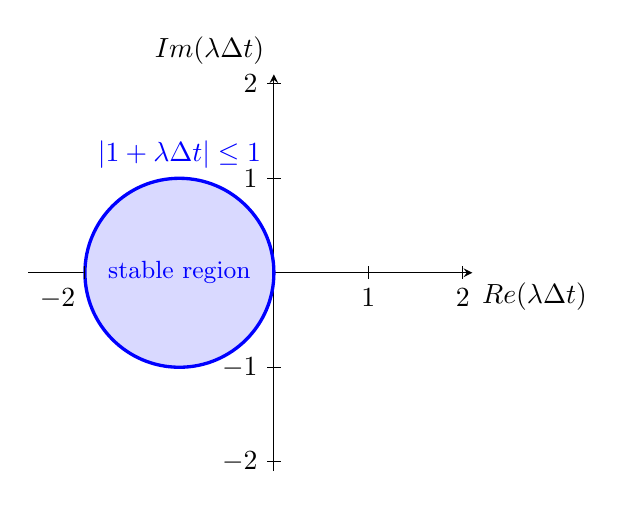
\begin{tikzpicture}[x=1.2cm,y=1.2cm,>=stealth]
        \draw[->] (-2.6,0) -- (2.1,0) node[below right] {$\operatorname{Re}(\lambda \Delta t)$};
        \draw[->] (0,-2.1) -- (0,2.1) node[above left] {$\operatorname{Im}(\lambda \Delta t)$};
    
        \foreach \x in {1,2}{
        \draw (\x,0) -- ++(0,0.07);
        \draw (\x,0) -- ++(0,-0.07) node[below] {$\x$};
        }
        \foreach \y in {-2,-1,1,2}{
        \draw (0,\y) -- ++(0.07,0);
        \draw (0,\y) -- ++(-0.07,0) node[left] {$\y$};
        }
    
        \filldraw[fill=blue!15,draw=blue,very thick] (-1,0) circle (1);
    
        \node[above,blue] at (-1,1) {$|1+\lambda\Delta t| \le 1$};
    
        \node[align=center,blue] at (-1,0) {\small stable region};
    
        \draw (-2,0) -- ++(0,0.07);
        \draw (-2,0) -- ++(0,-0.07) node[below left] {$-2$};
    
    \end{tikzpicture}
    \end{center}
    \caption{Region of absolute stability of forward (explicit) Euler: the unit disk centered at $-1$ in the $z=\lambda\Delta t$ plane.}\label{fig:euler-stability}
\end{figure}

So, the numerical method is only stable if the scaled step, $z_j = \lambda_j \Delta t$, falls \textit{inside} this circular region for all eigenvalues $\lambda_j$ of the system. This is a significant problem. The true system is stable for any $\lambda_j$ in the entire left-half of the complex plane ($\text{Re}(\lambda_j) \le 0$), but our numerical method is only stable for a small circular patch within that region. This means that even if the true solution is stable, our numerical solution can become unstable and explode if we choose a step size $\Delta t$ that is too large. This is known as conditional stability.

If $\lambda$ is real and negative (e.g., in a simple decay problem), we can define the characteristic time-scale of the problem as $\tau = -1/\lambda$. The stability condition becomes $|1 - \Delta t / \tau| \le 1$, which simplifies to
\begin{equation}
    0 \le \Delta t \le 2\tau
\end{equation}
The step size must be less than twice the characteristic time-scale of the system or the solution will become unstable.

\subsection{The Midpoint Method}

The forward Euler method is simple but has a large global error ($O(\Delta t)$) and a very restrictive stability region. We can develop more accurate methods. Let's consider another explicit method: the midpoint method. The midpoint method is a two-stage process. First, it takes a trial half-step using forward Euler to estimate the state at the midpoint of the time interval. Then, it uses the derivative at that estimated midpoint to take the full step from $t_i$ to $t_{i+1}$. This is visualized in \autoref{fig:midpoint-method-demo}.

\begin{definitionBox}
    \textbf{The Midpoint Method}

    Given $\mathbf{x}(t_i)$, find $\mathbf{x}(t_{i+1})$ by doing the following:
    \begin{enumerate}
        \item Estimate midpoint: $\mathbf{y} = \mathbf{x}(t_i) + \frac{\Delta t_i}{2} \mathbf{f}(\mathbf{x}(t_i), t_i)$
        \item Take full step: $\mathbf{x}(t_{i+1}) = \mathbf{x}(t_i) + \Delta t_i \mathbf{f}(\mathbf{y}, t_i + \Delta t_i/2)$
    \end{enumerate}
    This can be written in our general form $\mathbf{x}(t_{i+1}) = \mathbf{x}(t_i) + \Delta t_i \mathbf{g}(\mathbf{x}(t_i), t_i, \Delta t_i)$, where the function $\mathbf{g}$ is
    \begin{equation}
        \mathbf{g}(\mathbf{x}(t_i), t_i, \Delta t_i) = \mathbf{f}\left( \mathbf{x}(t_i) + \frac{\Delta t_i}{2}\mathbf{f}(\mathbf{x}(t_i), t_i), t_i + \Delta t_i/2 \right)
    \end{equation}
\end{definitionBox}

\begin{figure}[htbp]
    \begin{center}
        \begin{tikzpicture}[>=Stealth, line cap=round, line join=round, scale=0.9]

            \pgfmathdeclarefunction{f}{1}{\pgfmathparse{2.2*ln(#1+1)+0.3}}
            \pgfmathdeclarefunction{fp}{1}{\pgfmathparse{2.2/(#1+1)}}
            
            \pgfmathsetmacro{\tn}{3}
            \pgfmathsetmacro{\tm}{6}
            \pgfmathsetmacro{\tnp}{9}
            
            \pgfmathsetmacro{\yn}{f(\tn)}
            \pgfmathsetmacro{\ym}{f(\tm)}
            \pgfmathsetmacro{\slope}{fp(\tm)}
            \pgfmathsetmacro{\yend}{\yn + \slope*(\tnp-\tn)}
            
            \draw[->] (0,0) -- (10.5,0);
            
            \draw[very thick,blue] plot[domain=0.4:10, samples=200] (\x,{f(\x)});
            \node[blue] at (1.1,2.3) {$x(t)$};
            
            \foreach \x/\lab in {\tn/$t_i$, \tm/$t_i+\frac{\Delta t_i}{2}$, \tnp/$t_{i+1}$} {
            \draw[dashed] (\x,0) -- (\x,{f(\x)+0.4});
            \node[below] at (\x,-0.02) {\lab};
            }
            
            \draw[very thick,red] (\tn,\yn) -- (\tnp,\yend);
            \fill[red] (\tn,\yn) circle (2pt);
            \fill[red] (\tnp,\yend) circle (2pt);
            \node[red,anchor=south east] at (\tn,\yn) {$x_i$};
            \node[red,anchor=south west] at (\tnp,\yend) {$x_{i+1}$};

            \draw[very thick,purple!70!black] (\tm-2,{\ym-\slope*2}) -- (\tm+2.5,{\ym+\slope*2.5});
        
        \end{tikzpicture}
    \end{center}
    \caption{Midpoint method visualization. To improve over forward Euler, evaluate the derivative at the midpoint ($t_i+\Delta t_i/2$) (purple) and step from ($x_i$) to ($x_{i+1}$) (red) toward the exact solution ($x(t)$) (blue).}
    \label{fig:midpoint-method-demo}
\end{figure}

\paragraph*{Local Truncation Error of the Midpoint Method}

Let's estimate the LTE of this method. We need to compare the Taylor expansion of $\mathbf{g}$ with the Taylor expansion of the exact solution. First, let's expand $\mathbf{g}$ with respect to $\Delta t_i$ around $\Delta t_i = 0$:
\begin{align*}
    \mathbf{g}(\mathbf{x}(t_i), t_i, \Delta t_i) &= \mathbf{f}(\mathbf{x}(t_i), t_i) + \Delta t_i \frac{\partial \mathbf{g}}{\partial \Delta t_i}\bigg|_{\Delta t_i=0} + O(\Delta t_i^2) \\
    &= \mathbf{f}(\mathbf{x}(t_i), t_i) + \frac{\Delta t_i}{2} \frac{d\mathbf{f}}{dt}\bigg|_{\mathbf{x}(t_i), t_i} + O(\Delta t_i^2) \\
    &= \mathbf{f}(\mathbf{x}(t_i), t_i) + \frac{\Delta t_i}{2} \frac{d^2\mathbf{x}}{dt^2}\bigg|_{t_i} + O(\Delta t_i^2)
\end{align*}
Now, our numerical approximation is $\mathbf{x}(t_{i+1}) = \mathbf{x}(t_i) + \Delta t_i \mathbf{g}(\dots)$. Substituting our expansion for $\mathbf{g}$, we get
\begin{align*}
    \mathbf{x}(t_{i+1}) &= \mathbf{x}(t_i) + \Delta t_i \left( \mathbf{f}(\mathbf{x}(t_i), t_i) + \frac{\Delta t_i}{2} \frac{d^2\mathbf{x}}{dt^2}\bigg|_{t_i} + O(\Delta t_i^2) \right) \\
    &= \mathbf{x}(t_i) + \Delta t_i \mathbf{f}(\mathbf{x}(t_i), t_i) + \frac{(\Delta t_i)^2}{2} \frac{d^2\mathbf{x}}{dt^2}\bigg|_{t_i} + O(\Delta t_i^3)
\end{align*}
Compare this to the Taylor expansion of the \textit{exact} solution, we have
\begin{equation}
    \mathbf{x}_{\text{exact}}(t_{i+1}) = \mathbf{x}(t_i) + \Delta t_i \frac{d\mathbf{x}}{dt}\bigg|_{t_i} + \frac{(\Delta t_i)^2}{2} \frac{d^2\mathbf{x}}{dt^2}\bigg|_{t_i} + \frac{(\Delta t_i)^3}{6} \frac{d^3\mathbf{x}}{dt^3}\bigg|_{t_i} + \dots
\end{equation}
Since $\mathbf{f}(\mathbf{x}(t_i), t_i) = \frac{d\mathbf{x}}{dt}\big|_{t_i}$, we can see that the first three terms (the $O(1)$, $O(\Delta t_i)$, and $O(\Delta t_i^2)$ terms) of our numerical approximation and the exact solution match perfectly. The local truncation error $\epsilon = \| \mathbf{x}_{\text{exact}}(t_{i+1}) - \mathbf{x}(t_{i+1}) \|$ is therefore the first term that \textit{doesn't} match, which comes from the $O(\Delta t_i^3)$ term.
\begin{equation}
    \epsilon = \left\| \sum_{j=3}^{\infty} \frac{1}{j!} \Delta t_i^j \frac{d^j \mathbf{x}}{dt^j}\bigg|_{t_i} - \Delta t_i O(\Delta t_i^2) \right\| \sim O(\Delta t_i^3)
\end{equation}
This local error is one order higher than forward Euler's ($O(\Delta t_i^2)$). This means the global error of the midpoint method is $O(\Delta t^2)$, making it a second-order method.

\paragraph*{Stability of the Midpoint Method}
Let's analyze the stability of the midpoint method using the same ND test problem, $\mathbf{f}(\mathbf{x}(t), t) = \mathbf{A}\mathbf{x}(t)$. First, we find the intermediate step $\mathbf{y}$:
\begin{equation}
    \mathbf{y} = \mathbf{x}(t_i) + \frac{\Delta t_i}{2} \mathbf{A} \mathbf{x}(t_i) = \left(\mathbf{I} + \frac{\Delta t_i}{2} \mathbf{A}\right) \mathbf{x}(t_i)
\end{equation}
Next, we find the full step $\mathbf{x}(t_{i+1})$:
\begin{align}
    \mathbf{x}(t_{i+1}) &= \mathbf{x}(t_i) + \Delta t_i \mathbf{A} \mathbf{y} \nonumber \\
    &= \mathbf{x}(t_i) + \Delta t_i \mathbf{A} \left[ \left(\mathbf{I} + \frac{\Delta t_i}{2} \mathbf{A}\right) \mathbf{x}(t_i) \right] \nonumber \\
    &= \left[ \mathbf{I} + \Delta t_i \mathbf{A} + \frac{(\Delta t_i)^2}{2} \mathbf{A}^2 \right] \mathbf{x}(t_i)
\end{align}
Again, we can analyze this by looking at the eigenvalues $\lambda_j$ of $\mathbf{A}$. The stability condition for each decoupled component $y_j(t_i)$ is
\begin{equation}
    y_j(t_{i+1}) = \left[ 1 + \lambda_j \Delta t_i + \frac{(\lambda_j \Delta t_i)^2}{2} \right] y_j(t_i)
\end{equation}
For the numerical solution to be stable, the growth factor must have a magnitude less than or equal to 1. The condition is
\begin{equation}
    \left| 1 + \lambda_j \Delta t_i + \frac{(\lambda_j \Delta t_i)^2}{2} \right| \le 1
\end{equation}
Plotting this region in the complex plane shows a bean-like shape (see \autoref{fig:midpoint-stability}). The midpoint method has a larger stability region in the complex plane (its region strictly contains the forward Euler disk). However, along the negative real axis, both methods share the same stability interval $[0, 2/|\lambda|]$ for the scalar test problem. Note that purely imaginary eigenvalues (except at the origin) lie outside the stability region, which makes the midpoint method unsuitable for undamped oscillatory problems.

\begin{figure}[htbp]
    \centering
    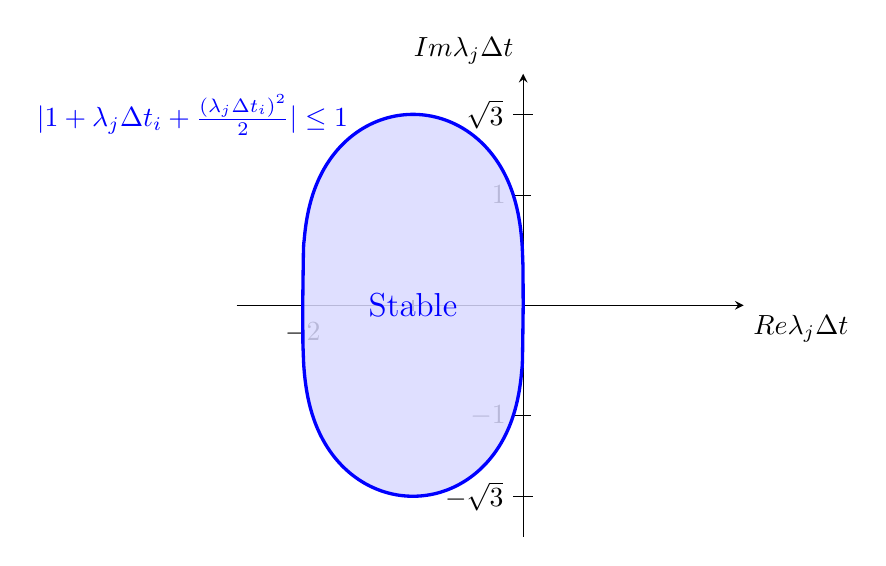
\begin{tikzpicture}[x=1.4cm,y=1.4cm,>=stealth]
      \draw[->] (-2.6,0) -- (2.0,0) node[below right] {$\operatorname{Re}\lambda_j\Delta t$};
      \draw[->] (0,-2.1) -- (0,2.1) node[above left] {$\operatorname{Im}\lambda_j\Delta t$};
    
      \foreach \y/\lab in {-1/{$-1$},1/{$1$}}{
        \draw (0,\y) -- ++(0.07,0);
        \draw (0,\y) -- ++(-0.07,0) node[left] {\lab};
      }
      \draw (0,{sqrt(3)}) -- ++(0.09,0);
      \draw (0,{sqrt(3)}) -- ++(-0.09,0) node[left] {$\sqrt{3}$};
      \draw (0,{-sqrt(3)}) -- ++(0.09,0);
      \draw (0,{-sqrt(3)}) -- ++(-0.09,0) node[left] {$-\sqrt{3}$};
    
      \draw (-2,0) -- ++(0,0.07);
      \draw (-2,0) -- ++(0,-0.07) node[below] {$-2$};
      \draw (-1,0) -- ++(0,0.05);
      \draw (-1,0) -- ++(0,-0.05);
    
      \path[fill=blue!15,fill opacity=.85,draw=blue,very thick]
        plot[domain=-2:0,samples=300,smooth]
          (\x,{ sqrt( -\x*(\x+2) + 2*sqrt(-\x*(\x+2)) ) })
        --
        plot[domain=0:-2,samples=300,smooth]
          (\x,{ -sqrt( -\x*(\x+2) + 2*sqrt(-\x*(\x+2)) ) })
        -- cycle;
    
      \node[blue] at (-1,0) {\large Stable};
    %   \node[align=center] at (-2.45,0.8) {Unstable};

        \node[above,blue] at (-3,1.45) {$|1+\lambda_j\Delta t_i + \frac{(\lambda_j\Delta t_i)^2}{2}| \le 1$};
    \end{tikzpicture}
    \caption{Region of absolute stability of the explicit midpoint method in the $z=\lambda_j\Delta t$ plane. The boundary passes through $z=-2,0$ and has extrema at $z=-1\pm i\sqrt{3}$.}
    \label{fig:midpoint-stability}
\end{figure}
    
\subsection{Comparing Explicit Methods: Euler vs.\ Midpoint}

We now have two methods: forward Euler (first-order, $O(\Delta t)$ global error) and midpoint (second-order, $O(\Delta t^2)$ global error). Let's compare them on the test problem
\begin{equation}
    \frac{dy}{dt} = -y, \qquad y(0)=1,
\end{equation}
whose exact solution is $y(t)=e^{-t}$.

\paragraph*{Accuracy at $t=1$ (global error vs.\ $\Delta t$).}
We measure the global error at a fixed time, $|y(1)-e^{-1}|$, while varying the step size $\Delta t$, and plot it on the log-log plot in \autoref{fig:global-error-comparison}. Forward Euler (red) has slope $\approx 1$ (error $\propto \Delta t$) and the midpoint method (blue) has slope $\approx 2$ (error $\propto \Delta t^2$). This means halving $\Delta t$ roughly halves the Euler error but quarters the midpoint error. Thus, for the same $\Delta t$, midpoint is significantly more accurate.

\begin{figure}[htbp]
    \centering
    \includegraphics[width=0.6\textwidth]{figs/ode/global_error_comparison.pdf}
    \caption{Global error at $t=1$ vs.\ $\Delta t$ (log--log). Forward Euler (red) shows first-order decay; midpoint (blue) shows second-order decay.}
    \label{fig:global-error-comparison}
\end{figure}

\paragraph*{Stability over time (solutions $y(t)$ for various $\Delta t$).}
\autoref{fig:stability-comparison} plots $y(t)$ produced by each method for several step sizes; the true solution is the dotted black curve. For small steps (e.g., $\Delta t=0.01,\,0.05,\,0.65$) both methods track $e^{-t}$ well. The stability question becomes interesting near the boundary:
\[
\text{Forward Euler:}\quad r_E(\Delta t)=1-\Delta t,\qquad
\text{Midpoint:}\quad r_M(\Delta t)=1-\Delta t+\tfrac12\Delta t^2
\]
For this scalar test with $\lambda=-1$, absolute stability requires $|r(\Delta t)|\le 1$, which holds for $0\le \Delta t\le 2$ for \emph{both} methods. At the edge,
\begin{itemize}
    \item \(\Delta t=2\): Euler is marginally stable with $r_E=-1 \implies y_n=(-1)^n$ (alternating, no decay); midpoint is marginally stable with $r_M=1 \implies y_n = 1$ (flat, no decay).
    \item \(\Delta t>2\) (e.g., $2.5$): both methods are unstable and the numerical solutions diverge.
\end{itemize}
Thus, for this problem, the stable interval on the negative real axis is the same (\(\Delta t\le 2\)), but the qualitative behavior at the boundary differs. Euler flips sign each step while midpoint holds its value. To obtain asymptotic decay toward zero (as desired), we need $\Delta t<2$.

\begin{figure}[htbp]
    \centering
    \includegraphics[width=0.6\textwidth]{figs/ode/stability_comparison.pdf}
    \caption{Time-series stability comparison. The exact solution (dotted black) and numerical solutions for several $\Delta t$ values; colors encode $\Delta t$, with solid lines for Euler and dashed lines for midpoint. At $\Delta t=2$ both methods are marginal (no decay); at $\Delta t=2.5$ both diverge.}
    \label{fig:stability-comparison}
\end{figure}



\subsection{Runge-Kutta Methods}

The explicit/forward Euler method and the midpoint method are both examples of a much broader and more powerful class of numerical integrators called Runge-Kutta (RK) methods. These methods are the go-to explicit methods for solving ODE-IVPs. They work by computing one or more intermediate stages (like the $\mathbf{y}$ vector in the midpoint method) and then using a weighted average of the derivatives at these stages to compute the final step.

An $s$-stage explicit Runge-Kutta method computes $\mathbf{x}(t_{i+1})$ from $\mathbf{x}(t_i)$ as follows:
\begin{equation}
    \mathbf{x}(t_{i+1}) = \mathbf{x}(t_i) + \Delta t_i \sum_{j=1}^{s} b_j \mathbf{k}_j
\end{equation}
where each stage $\mathbf{k}_j$ is a derivative evaluation:
\begin{equation}
    \mathbf{k}_j = \mathbf{f}\left( \mathbf{x}(t_i) + \Delta t_i \sum_{k=1}^{j-1} a_{jk} \mathbf{k}_k, t_i + c_j \Delta t_i \right)
\end{equation}
The method is defined by the set of coefficients: the weights $\mathbf{b} = (b_j)$, the node times $\mathbf{c} = (c_j)$, and the internal stage matrix $\mathbf{A} = (a_{jk})$. For explicit methods, $\mathbf{A}$ is strictly lower triangular ($a_{jk} = 0$ for $k \ge j$). We also require $\sum_{k=1}^{j-1} a_{jk} = c_j$ for $j=2, \dots, s$.

The coefficients $\mathbf{a}$, $\mathbf{b}$, and $\mathbf{c}$ are chosen (usually represented in something called a Butcher tableau) to minimize the local truncation error by matching as many terms as possible in the Taylor series expansion of the true solution. An $s$-stage RK method can achieve order $p$ by satisfying the RK order conditions; the resulting LTE is $O(\Delta t^{p+1})$ and global error is $O(\Delta t^{p})$. For explicit RK methods, higher order generally requires more stages (e.g., order 5 typically needs $\ge 6$ stages). For example, the forward Euler method is a 1-stage RK method ($s=1$) with $b_1=1$ and $c_1=0$ that achieves $O(\Delta t)$ global error. The midpoint method is a 2-stage RK method ($s=2$) with coefficients $b_1=0, b_2=1$, $c_1=0, c_2=1/2$, and $a_{21}=1/2$, which achieves $O(\Delta t^2)$ global error. A well-known example is RK4 (Runge-Kutta 4th-order), which uses 4 stages ($s=4$) to achieve a very accurate global error of $O(\Delta t^4)$ and is extremely common in engineering applications.


\section{Implicit Methods for Solving ODE-IVPs}

So far, we have looked at explicit methods where the future state $\mathbf{x}(t_{i+1})$ is calculated directly from known information at the current or previous time steps. While explicit methods are easy to implement and computationally cheap per step, we found that their stability regions are bounded. This imposes a strict limit on the step size $\Delta t$; if the step is too large, the solution explodes, even if the physics of the problem are stable. To overcome this stability limitation, we turn to \textbf{implicit methods}. The idea behind these methods is different: we approximate the solution at $t_{i+1}$ using knowledge of the solution at $t_i$ \textit{and} the unknown solution at $t_{i+1}$ itself. The general form for such a method is
\begin{equation}
    \mathbf{x}(t_{i+1}) = \mathbf{x}(t_i) + \Delta t_i \mathbf{g}(\mathbf{x}(t_{i+1}), \mathbf{x}(t_i), t_{i+1}, t_i, \Delta t_i)
\end{equation}
The main difference from explicit methods is that $\mathbf{x}(t_{i+1})$ appears on both sides of the equation (inside the function $\mathbf{g}$). This means we have to \textit{solve} for $\mathbf{x}(t_{i+1})$ rather than just plug in numbers. As with explicit methods, the step size $\Delta t_i$ controls the local truncation error, and the function $\mathbf{g}$ is designed to minimize this error.

\subsection{The Implicit (Backward) Euler Method}

The simplest implicit method is the implicit Euler (or backward Euler) method. Recall that explicit Euler used the derivative at the \textit{start} of the interval. Implicit Euler uses the derivative at the \textit{end} of the interval:
\begin{equation}
    \mathbf{x}(t_{i+1}) = \mathbf{x}(t_i) + \Delta t_i \mathbf{f}(\mathbf{x}(t_{i+1}), t_{i+1})
\end{equation}
This formula is derived from the finite difference approximation of the derivative $\mathbf{x}'(t)$ at time $t_{i+1}$, rather than $t_i$. To visualize the difference between the explicit and implicit Euler methods, it is helpful to view the ODE as an integration problem. Since $\frac{d\mathbf{x}}{dt} = \mathbf{f}(\mathbf{x}(t), t)$, we have
\begin{equation}
    \mathbf{x}(t_{i+1}) = \mathbf{x}(t_i) + \int_{t_i}^{t_{i+1}} \mathbf{f}(\mathbf{x}(t), t) dt
\end{equation}
If we \textit{conceptually} simplify $\mathbf{f}(\mathbf{x}(t), t)$ to a function of time $\mathbf{f}(t)$ (ignoring the $\mathbf{x}$ dependence for a moment to visualize), we can relate the ODE solvers to Riemann sums: explicit Euler approximates the integral using the rectangle rule with the left endpoint ($t_i$), which corresponds to a left Riemann sum. Meanwhile, implicit Euler approximates the integral using the rectangle rule with the right endpoint ($t_{i+1}$), which corresponds to a right Riemann sum. Note that this is just for intuition; formally $\mathbf{f}$ depends on $\mathbf{x}$, which is what makes the method implicit.

\begin{exampleBox}
    \textbf{Explicit vs.\ Implicit Euler:} Consider a simple scalar example: $x' = -x$.
    The explicit Euler method gives
    \begin{equation}
        x_{i+1} = x_i + \Delta t (-x_i) = (1-\Delta t)x_i
    \end{equation}
    The implicit Euler method gives
    \begin{equation}
        x_{i+1} = x_i + \Delta t (-x_{i+1})
    \end{equation}
    In the implicit case, we must rearrange to find $x_{i+1}$:
    \begin{equation}
        x_{i+1} (1 + \Delta t) = x_i \implies x_{i+1} = \frac{x_i}{1 + \Delta t}
    \end{equation}
\end{exampleBox}

\paragraph*{Accuracy of Implicit Euler}
We estimate the LTE for implicit Euler just as we did for the explicit case. The Taylor expansion of the exact solution around $t_{i+1}$ is
\begin{equation}
    \mathbf{x}_{\text{exact}}(t_i) = \mathbf{x}_{\text{exact}}(t_{i+1}) - \Delta t_i \frac{d\mathbf{x}}{dt}\bigg|_{t_{i+1}} + O(\Delta t_i^2)
\end{equation}
Rearranging for $\mathbf{x}_{\text{exact}}(t_{i+1})$ and substituting $\frac{d\mathbf{x}}{dt} = \mathbf{f}(\mathbf{x}, t)$, we get
\begin{equation}
    \mathbf{x}_{\text{exact}}(t_{i+1}) = \mathbf{x}_{\text{exact}}(t_i) + \Delta t_i \mathbf{f}(\mathbf{x}_{\text{exact}}(t_{i+1}), t_{i+1}) + O(\Delta t_i^2)
\end{equation}
Comparing this to the numerical formula, the local truncation error is
\begin{equation}
    \epsilon = \| \mathbf{x}_{\text{exact}}(t_{i+1}) - \mathbf{x}(t_{i+1}) \| \sim O(\Delta t_i^2)
\end{equation}
As $\Delta t_i \to 0$, the ratio $\epsilon / \Delta t_i^2 \to C > 0$. (That is, there exists a constant $C$ such that $\epsilon \approx C \Delta t_i^2$ for sufficiently small step sizes). Just like explicit Euler, the local error is quadratic ($O(\Delta t^2)$) and the global accumulated error is linear ($O(\Delta t)$). It is a first-order method. Note that because we sum $N \sim T/\Delta t$ steps, the global error is one order lower than the local error.

\paragraph*{Computational Cost: Solving the Nonlinear Equations}
If implicit Euler has the same accuracy as explicit Euler, why use it? The answer lies in stability (discussed below), but first, we must address the cost. In explicit Euler, calculating $\mathbf{x}(t_{i+1})$ is a simple plug-and-chug operation. In implicit Euler, $\mathbf{x}(t_{i+1})$ is defined implicitly:
\begin{equation}
    \mathbf{x}(t_{i+1}) - \Delta t_i \mathbf{f}(\mathbf{x}(t_{i+1}), t_{i+1}) - \mathbf{x}(t_i) = 0
\end{equation}
For a general nonlinear ODE, this requires solving a system of nonlinear algebraic equations at \textit{every single time step}. Let the unknown be $\mathbf{y} = \mathbf{x}(t_{i+1})$. We are looking for the root of the residual function:
\begin{equation}
    \mathbf{r}(\mathbf{y}) = \mathbf{y} - \Delta t_i \mathbf{f}(\mathbf{y}, t_{i+1}) - \mathbf{x}(t_i) = 0
\end{equation}
This is typically solved using Newton's method (of course!). Let's recall the scalar Newton iteration for finding a root $r(y)=0$:
\begin{equation}
    y^{(k+1)} = y^{(k)} - \frac{r(y^{(k)})}{r'(y^{(k)})}
\end{equation}
Generalizing to the vector case, we update an initial guess $\mathbf{y}^{(0)}$ by solving a linear system for the update $\Delta \mathbf{y}$:
\begin{equation}
    \mathbf{J}(\mathbf{y}^{(k)}) \Delta \mathbf{y} = -\mathbf{r}(\mathbf{y}^{(k)})
\end{equation}
and then applying it:
\begin{equation}
    \mathbf{y}^{(k+1)} = \mathbf{y}^{(k)} + \Delta \mathbf{y}
\end{equation}
where $\mathbf{J}$ is the Jacobian of the residual system:
\begin{equation}
    \mathbf{J} = \frac{\partial \mathbf{r}}{\partial \mathbf{y}} = \mathbf{I} - \Delta t_i \nabla_{\mathbf{y}} \mathbf{f}(\mathbf{y}, t_{i+1})
\end{equation}

\paragraph*{Practical Details.} 
First, a good guess speeds up convergence. We usually use the solution from the previous step ($\mathbf{y}^{(0)} = \mathbf{x}(t_i)$) or an explicit Euler prediction ($\mathbf{y}^{(0)} = \mathbf{x}(t_i) + \Delta t_i \mathbf{f}(\mathbf{x}(t_i), t_i)$). Second, the cost of solving the linear system is $O(N^3)$ (using Gaussian elimination/LU). Third, if the ODE is linear ($\mathbf{f} = \mathbf{A}\mathbf{x}$), the Jacobian $\mathbf{J} = \mathbf{I} - \Delta t_i \mathbf{A}$ is constant (for fixed $\Delta t$). You only need to factorize it once and can reuse the LU factors, making it much cheaper.

This makes implicit methods much more computationally expensive per step than explicit methods. We have to evaluate the Jacobian and solve a linear system multiple times per time step. However, as we will see, the stability properties allow us to take much larger steps.

\begin{warningBox}
    \textbf{The Hidden Cost of Implicit Methods:} Implicit methods provide stability, but they trade computational effort for it. In explicit Euler, calculating $\mathbf{x}_{i+1}$ is a direct formula evaluation. In implicit Euler, $\mathbf{x}_{i+1}$ is trapped inside a nonlinear function. 
    
    Finding $\mathbf{x}_{i+1}$ requires solving a root-finding problem $\mathbf{r}(\mathbf{y}) = 0$ at \textbf{every single time step}. This usually requires an iterative solver like Newton's Method, which involves:
    \begin{enumerate}
        \item Evaluating the Jacobian matrix $\mathbf{J}$.
        \item Solving a linear system $\mathbf{J} \Delta \mathbf{y} = -\mathbf{r}$.
    \end{enumerate}
    Consequently, one implicit step is much more expensive (in CPU time) than one explicit step. We only use implicit methods when the stability restriction on explicit methods forces the step size $\Delta t$ to be impractically small (i.e., stiff problems).
\end{warningBox}

\subsection{Stability of Implicit Euler}
We analyze the stability using the prototype linear problem $\dot{\mathbf{x}} = \mathbf{A}\mathbf{x}$. Applying the implicit formula,
\begin{equation}
    \mathbf{x}(t_{i+1}) = \mathbf{x}(t_i) + \Delta t_i \mathbf{A} \mathbf{x}(t_{i+1})
\end{equation}
Rearranging to solve for $\mathbf{x}(t_{i+1})$,
\begin{align}
    (\mathbf{I} - \Delta t_i \mathbf{A}) \mathbf{x}(t_{i+1}) &= \mathbf{x}(t_i) \\
    \mathbf{x}(t_{i+1}) &= (\mathbf{I} - \Delta t_i \mathbf{A})^{-1} \mathbf{x}(t_i)
\end{align}
Decoupling the system using the eigenvalues $\lambda_j$ of $\mathbf{A}$, the relationship for each component $y_j$ is
\begin{equation}
    y_j(t_{i+1}) = (1 - \Delta t_i \lambda_j)^{-1} y_j(t_i)
\end{equation}
For stability, we require the magnitude of the amplification factor to be less than or equal to 1:
\begin{equation}
    \left| \frac{y_j(t_{i+1})}{y_j(t_i)} \right| = \left| (1 - \Delta t_i \lambda_j)^{-1} \right| \le 1
\end{equation}
It is helpful to define the complex variable $z = \lambda \Delta t$ and the stability function $R(z) = (1-z)^{-1}$. The condition becomes $|R(z)| \le 1$, or
\begin{equation}
    |1 - z| \ge 1
\end{equation}
Expanding this with $z = x + iy$, we get
\begin{equation}
    |(1 - z)|^2 = (1 - x)^2 + y^2 \ge 1
\end{equation}
Geometrically, $|1-z|=1$ is a circle in the complex plane with radius 1 centered at $z=+1$. The stability condition $|1-z| \ge 1$ is satisfied everywhere \textit{outside} this circle.
Since the entire left half-plane ($\text{Re}(z) \le 0$) lies outside this circle, implicit Euler is stable for any stable linear system, regardless of the step size.

\begin{definitionBox}
    \textbf{A-Stability}
    
    A numerical method is called \textbf{A-stable} if its region of absolute stability includes the entire left half-plane of the complex numbers ($\text{Re}(z) \le 0$). This means that if the exact solution decays ($\text{Re}(\lambda) < 0$), the numerical solution will also decay for \emph{any} step size $\Delta t > 0$. Implicit Euler is A-stable. Explicit Euler is not.
\end{definitionBox}
The region of stability for implicit Euler is shown in \autoref{fig:implicit_euler_stability}.

\begin{figure}[H]
    \centering
    \includegraphics[width=0.4\textwidth]{figs/ode/implicit_euler_stability.pdf}
    \caption{Implicit Euler stability region. Unlike explicit Euler, which was only stable inside a small circle, implicit Euler is stable everywhere outside the small white circle. It is stable for the entire left half-plane.}
    \label{fig:implicit_euler_stability}
\end{figure}

Importantly, if the real part of $\lambda_j$ is negative (which corresponds to a stable physical system where the true solution decays), implicit Euler is always stable, regardless of the step size $\Delta t_i$. This property is extremely powerful.

\subsection{The Crank-Nicolson Method}

We can improve the accuracy of the implicit approach by combining the ideas of the trapezoidal rule for integration. The Crank-Nicolson method averages the slope at the beginning and the end of the interval:
\begin{equation}
    \mathbf{x}(t_{i+1}) = \mathbf{x}(t_i) + \frac{\Delta t_i}{2} \left[ \mathbf{f}(\mathbf{x}(t_{i+1}), t_{i+1}) + \mathbf{f}(\mathbf{x}(t_i), t_i) \right]
\end{equation}
Or, written in our general form,
\begin{equation}
    \mathbf{g}(\dots) = \frac{1}{2} \left[ \mathbf{f}(\mathbf{x}(t_{i+1}), t_{i+1}) + \mathbf{f}(\mathbf{x}(t_i), t_i) \right]
\end{equation}
This corresponds to the trapezoidal rule for integration. Because of this, the method is called the implicit trapezoidal rule.

% \begin{exampleBox}
%     \textbf{Summary: Crank-Nicolson}
%     \begin{itemize}
%         \item \textbf{Method:} Implicit Trapezoidal Rule.
%         \item \textbf{Accuracy:} LTE is $O(\Delta t^3)$, Global Error is $O(\Delta t^2)$ (Second-Order).
%         \item \textbf{Stability:} A-stable (stable in entire left half-plane), but not L-stable (see ringing below).
%     \end{itemize}
% \end{exampleBox}

\paragraph*{Accuracy of Crank-Nicolson}
Estimating the local truncation error via Taylor expansion shows that
\begin{equation}
    \mathbf{x}(t_{i+1}) \approx \mathbf{x}(t_i) + \Delta t_i \mathbf{f}(t_i) + \frac{\Delta t_i^2}{2} \mathbf{f}'(t_i) + O(\Delta t_i^3)
\end{equation}
That is, the local truncation error is $O(\Delta t_i^3)$. Consequently, the global truncation error is $O(\Delta t^2)$. Crank-Nicolson is thus a second-order method, meaning that it has better accuracy than implicit Euler while maintaining implicit properties.

\paragraph*{Stability of Crank-Nicolson}
Applying the method to the prototype problem $\dot{\mathbf{x}} = \mathbf{A}\mathbf{x}$,
\begin{equation}
    \mathbf{x}(t_{i+1}) = \mathbf{x}(t_i) + \frac{\Delta t_i}{2} \mathbf{A} (\mathbf{x}(t_{i+1}) + \mathbf{x}(t_i))
\end{equation}
Rearranging terms to group $\mathbf{x}(t_{i+1})$ on the left and $\mathbf{x}(t_i)$ on the right,
\begin{equation}
    \left[ \mathbf{I} - \frac{\Delta t_i}{2} \mathbf{A} \right] \mathbf{x}(t_{i+1}) = \left[ \mathbf{I} + \frac{\Delta t_i}{2} \mathbf{A} \right] \mathbf{x}(t_i)
\end{equation}
For a component $y_j$ corresponding to eigenvalue $\lambda_j$, we have
\begin{equation}
    y_j(t_{i+1}) = \left( 1 - \frac{\Delta t_i \lambda_j}{2} \right)^{-1} \left( 1 + \frac{\Delta t_i \lambda_j}{2} \right) y_j(t_i)
\end{equation}
The stability condition is
\begin{equation}
    \left| \frac{1 + \frac{\Delta t_i \lambda_j}{2}}{1 - \frac{\Delta t_i \lambda_j}{2}} \right| \le 1
\end{equation}
To see why, let $z = \frac{\Delta t_i \lambda_j}{2} = a + ib$. Then the condition is
\begin{equation}
    \left| \frac{1+z}{1-z} \right| \le 1 \iff |1+z|^2 \le |1-z|^2
\end{equation}
Substituting $z=a+ib$, we have
\begin{align}
    (1+a)^2 + b^2 &\le (1-a)^2 + b^2 \\
    1 + 2a + a^2 + b^2 &\le 1 - 2a + a^2 + b^2 \\
    4a &\le 0 \implies a \le 0
\end{align}
Since $a = \text{Re}(z) = \frac{\Delta t_i}{2} \text{Re}(\lambda_j)$, this inequality holds whenever $\text{Re}(\lambda_j) \le 0$. Thus, Crank-Nicolson is A-stable, meaning its stability region includes the entire left half-plane.

\begin{figure}[H]
    \centering
    \includegraphics[width=0.6\textwidth]{figs/ode/crank_nicolson_stability.pdf}
    \caption{Stability region of the Crank-Nicolson method. The method is stable for all eigenvalues with a negative real part (the entire left half-plane).}
    \label{fig:cn_stability}
\end{figure}

\subsection{Comparison of Implicit Behavior}
While both implicit Euler and Crank-Nicolson are stable in the left half-plane, their behavior for very large step sizes differs. Consider the simple scalar decay equation $dy/dt = -y$ (where $\lambda = -1$). For implicit Euler, as $\Delta t \to \infty$, the amplification factor $(1 - \lambda \Delta t)^{-1} \to 0$. The numerical solution decays smoothly to zero, matching the physics. For Crank-Nicolson, as $\Delta t \to \infty$, the amplification factor approaches $\frac{\lambda \Delta t / 2}{-\lambda \Delta t / 2} = -1$. The solution does not explode, but it oscillates between $+1$ and $-1$ without decaying. This oscillatory behavior (ringing) in Crank-Nicolson can be problematic for very stiff systems (the concept of stiffness will be discussed momentarily) where high-frequency components should decay rapidly but instead persist as numerical noise.

\begin{exampleBox}
    % MC: I think this is not the best example of the behavior, should probably change to something more clear
    \textbf{Stability vs. Monotonicity (Ringing)}
    
    Consider the decay equation $y' = -y$ (exact solution $e^{-t}$). While both implicit Euler and Crank-Nicolson are unconditionally stable (the solution does not explode, see \autoref{fig:cn_stability}), they behave very differently for large time steps (e.g., $\Delta t = 10$).

    \textbf{1. Implicit Euler (Smooth Decay)}
    The update rule is $y_{i+1} = \frac{1}{1 + \Delta t} y_i$. Note that the denominator is always positive. For $\Delta t = 10$,
    \begin{equation*}
        y_{i+1} = \frac{1}{11} y_i \approx 0.09 y_i
    \end{equation*}
    The solution remains positive and decays monotonically, matching the physics.

    \textbf{2. Crank-Nicolson (Oscillation)}
    The update rule is $y_{i+1} = \frac{2 - \Delta t}{2 + \Delta t} y_i$. If $\Delta t > 2$, the numerator becomes negative. For $\Delta t = 10$,
    \begin{equation*}
        y_{i+1} = \frac{2 - 10}{2 + 10} y_i = -\frac{2}{3} y_i \approx -0.67 y_i
    \end{equation*}
    The magnitude decreases ($0.67 < 1$, so it is stable), but the sign flips at every step. This artificial oscillation is called ringing.

    \begin{figure}[H]
        \centering
        \includegraphics[width=0.7\textwidth]{figs/ode/implicit_comparison_example.pdf}
        \caption{Implicit stability example solving $y' = -y$. While both methods are stable, Crank-Nicolson (dashed) can exhibit oscillations for large time steps $\Delta t$, whereas implicit Euler (solid) decays monotonically.}
        \label{fig:implicit_comparison}
    \end{figure}
\end{exampleBox}

\begin{definitionBox}
    \textbf{L-Stability}
    
    A method is \textbf{L-stable} if it is A-stable \textit{and} the amplification factor approaches 0 as the step size goes to infinity:
    \begin{equation}
        \lim_{|z| \to \infty} |R(z)| = 0 \quad (\text{for } \text{Re}(z) < 0)
    \end{equation}
    Methods that are L-stable (like implicit Euler) quickly damp out high-frequency noise/transients. Methods that are A-stable but not L-stable (like Crank-Nicolson, where $|R(z)| \to 1$) can allow high-frequency noise to persist as ringing.
\end{definitionBox}

\subsection{Revisiting the Prototype Problem}
To formalize these observations, let us look again at the prototype problem:
\begin{equation}
    \frac{d\mathbf{x}}{dt} = \mathbf{A}\mathbf{x}(t), \quad \mathbf{x}(0) = \mathbf{x}_0
\end{equation}
The exact solution is $\mathbf{x}(t) = \mathbf{W}^{-1} e^{\boldsymbol{\Lambda} t} \mathbf{W} \mathbf{x}_0$. The system is analytically stable if $\text{Re}(\lambda_i) \le 0$ for all $i = 1, \dots, N$.
The system dynamics are characterized by time constants $\tau_i = |\lambda_i^{-1}|$. If we have a system where the time constants are roughly the same magnitude, explicit methods work well. However, consider what happens when the ratio of the largest to smallest time constant is very large:
\begin{equation}
    \frac{\tau_{\max}}{\tau_{\min}} \gg 1 \quad \text{or} \quad \frac{|\lambda|_{\max}}{|\lambda|_{\min}} \gg 1
\end{equation}
This situation implies the solution spans a wide range of time scales. The fast modes (small $\tau$) decay very quickly, but to capture them stably with an explicit method, $\Delta t$ must be very small. However, we likely want to simulate the system long enough to see the slow modes (large $\tau$) evolve. This forces us to take an exorbitant number of tiny steps. This specific difficulty is known as stiffness, which we discuss next.

\section{Stiff Differential Equations}

In the previous section on implicit methods, we alluded to a class of problems where the stability constraints of explicit methods become prohibitive. These are known as \textbf{stiff equations}. Stiffness usually arises in systems where physical phenomena occurring at widely varying time scales are coupled together. For example, a chemical reaction might involve one intermediate species that reacts in microseconds, while the overall product forms over minutes. To resolve the fast reaction explicitly, the time step $\Delta t$ must be on the order of microseconds. However, to simulate the full process, we need to take millions of those tiny steps, even after the fast transient has died out and the system is evolving slowly.

We can characterize stiffness by the ratio of the largest to the smallest time constants in the system. For a linear system with eigenvalues $\lambda_i$, for decaying modes, $\tau_i \approx -1/\text{Re}(\lambda_i)$; for real negative $\lambda_i$, this is proportional to $1/|\lambda_i|$. From this, we see that the ratio of time constants is equivalent to the ratio of eigenvalue magnitudes:
\begin{equation}
    \text{Stiffness} \sim \frac{\max |\lambda_i|}{\min |\lambda_i|} \approx \frac{\tau_{\max}}{\tau_{\min}}
\end{equation}
Alternatively, considering the simulation duration $t_f$, the difficulty is proportional to $t_f / \tau_{\min}$.

The conflict in stiff problems is fundamental. Explicit solvers require $\Delta t$ to be bounded by the smallest time constant ($\Delta t < C \tau_{\min}$) to prevent explosion. However, if $\tau_{\min} \ll t_f$, the number of steps $N_{\text{steps}} = t_f / \Delta t$ becomes enormous. Furthermore, each of these steps adds a small amount of finite-precision floating point error to the state vector. If we take too many steps, the accumulated round-off error destroys accuracy.

Some implicit methods, such as backward Euler and the trapezoidal rule, possess the property of A-stability. An A-stable method has a stability region that contains the entire left half of the complex plane ($\text{Re}(z)<0$ for $z = \lambda \Delta t$), so it doesn't impose a stability step-size restriction on decaying modes. They allow the step size $\Delta t$ to be chosen based on the accuracy required to track the solution's curvature rather than being dictated by the fastest decaying mode. While each implicit step is more expensive (requiring a Jacobian solve), the ability to take steps orders of magnitude larger makes them the only viable choice for stiff problems.

\begin{exampleBox}
    \textbf{Example: Stiff Coupled System.}
    Consider:
    \begin{equation}
        y_1' = -y_1, \quad y_2' = -1000 y_2
    \end{equation}
    Here, $\lambda_1 = -1$ (slow) and $\lambda_2 = -1000$ (fast). Explicit Euler requires $|1 + \lambda \Delta t| \le 1$. For $\lambda_2 = -1000$, we need $|1 - 1000 \Delta t| \le 1 \implies \Delta t \le 0.002$. The update for the fast mode is $y_{n+1} = (1 - 1000 \Delta t)y_n$. If we choose $\Delta t=0.1$, the amplification factor is $(1 - 100) = -99$, so the error grows by $99\times$ each step, causing explosion.

    On the other hand, implicit Euler is stable for any $\Delta t$. The update is $y_{n+1} = \frac{1}{1 - \lambda \Delta t} y_n$. For $\Delta t = 0.1$ and $\lambda = -1000$, the amplification factor is $\frac{1}{1 + 100} \approx 0.01$. The fast mode decays rapidly to zero, as it should physically. We can safely choose $\Delta t = 0.1$ to capture the slow evolution of $y_1$ without worry.
\end{exampleBox}

\begin{exampleBox}
    \textbf{Example: The Van der Pol Oscillator}
    A classic example of a stiff system is the Van der Pol oscillator with a large nonlinearity parameter that we call $\lambda$ here. The governing equations are
    \begin{equation}
        \frac{d\mathbf{x}}{dt} = \begin{bmatrix} \dot{x}_1 \\ \dot{x}_2 \end{bmatrix} = \begin{bmatrix} x_2 \\ \lambda(1 - x_1^2)x_2 - x_1 \end{bmatrix}
    \end{equation}
    When $\lambda$ is large, the damping term $\lambda(1-x_1^2)x_2$ dominates. To analyze the stiffness, we define a perturbation $\delta \mathbf{x} = \mathbf{x} - \mathbf{x}^*$. Linearizing the dynamics around $\mathbf{x}^*$ gives
    \begin{equation}
        \frac{d}{dt} \delta\mathbf{x} \approx \mathbf{J}(\mathbf{x}^*) \delta\mathbf{x} = \begin{bmatrix} 0 & 1 \\ -2\lambda x_1^* x_2^* - 1 & \lambda(1 - (x_1^*)^2) \end{bmatrix} \delta\mathbf{x}
    \end{equation}
    Consider the state where the system passes through $x_1 \approx 0$. The Jacobian becomes:
    \begin{equation}
        \mathbf{J} \approx \begin{bmatrix} 0 & 1 \\ -1 & \lambda \end{bmatrix}
    \end{equation}
    The eigenvalues $\mu$ satisfy $\mu^2 - \lambda \mu + 1 = 0$, which implies $\mu \approx \lambda$ and $\mu \approx 1/\lambda$ for large $\lambda$. The corresponding time constants are $T_{\max} \approx \lambda$ and $T_{\min} \approx 1/\lambda$. The stiffness ratio scales as:
    \begin{equation}
        \frac{T_{\max}}{T_{\min}} \sim \frac{\lambda}{1/\lambda} = O(\lambda^2)
    \end{equation}
    Physically, the solution rapidly traverses the fast segments (associated with the large eigenvalue $\sim \lambda$) and then slowly drifts along the slow manifold (time scale $\sim \lambda$). A nonstiff solver must use tiny steps everywhere because of the brief fast phases. For $\lambda = 100$, the stiffness ratio is $10,000$. An explicit solver would require steps 10,000 times smaller than the slow dynamics suggest.

    \begin{figure}[H]
        \centering
        \includegraphics[width=0.8\textwidth]{figs/ode/stiff_comparison.pdf}
        \caption{Numerical solution of the stiff Van der Pol oscillator with $\lambda = 100$ using a nonstiff explicit solver (ode45 / RK45, blue) and a stiff implicit solver (ode15s / Radau, red). Both methods trace the same limit cycle in $x_1(t)$, but the stiff solver uses far fewer, adaptively placed time steps and function evaluations (see statistics box), making it substantially more efficient for this stiff problem.}
        \label{fig:stiffness_vdp}
    \end{figure}
\end{exampleBox}

\section{\texorpdfstring{Adaptive Time Stepping\textsuperscript{*}}{Adaptive Time Stepping}}

In practical applications, we rarely use a fixed step size $\Delta t$. The solution may vary slowly for long periods (allowing large steps) and then change rapidly (requiring small steps). To handle this, we employ adaptive time stepping. The goal is to choose $\Delta t_i$ such that the LTE is kept below a user-specified tolerance $\epsilon$. Since we do not know the exact solution, we must estimate the error using available data. A common strategy involves using the properties of the numerical method itself. Consider the explicit midpoint method we discussed earlier:
\begin{align}
    \mathbf{y} &= \mathbf{x}_i + \frac{\Delta t_i}{2} \mathbf{f}(\mathbf{x}_i, t_i) \\
    \mathbf{x}_{i+1} &= \mathbf{x}_i + \Delta t_i \mathbf{f}(\mathbf{y}, t_i + \Delta t_i/2)
\end{align}
As part of the error estimate, we additionally evaluate the function at the end of the step, $\mathbf{f}(\mathbf{x}_{i+1}, t_{i+1})$, giving us three values of $\mathbf{f}$ over the step (start, midpoint, and end). It can be shown via Taylor expansion that a linear combination of these evaluations acts as a proxy for the LTE:
\begin{equation}
    \text{Error Proxy} \approx \Delta t_i \left[ \mathbf{f}(\mathbf{x}_i, t_i) + \mathbf{f}(\mathbf{x}_{i+1}, t_{i+1}) - 2\mathbf{f}(\mathbf{y}, t_i + \Delta t_i/2) \right] \sim O(\Delta t_i^3)
\end{equation}
This quantity acts as an error indicator (conceptually proportional to $\Delta t^3$ times the curvature of $\mathbf{f}$ along the step). If the function were perfectly linear, this term would vanish.

\paragraph*{\texorpdfstring{Adaptive Step Algorithm\textsuperscript{*}}{Adaptive Step Algorithm}}
The adaptive procedure works by first computing the trial step to get $\mathbf{x}_{i+1}$ and then calculating the error estimate $\mathbf{E} = \| \Delta t_i [\dots] \|_2$. We then check if this error satisfies the tolerance condition $\mathbf{E} \le \epsilon_a + \epsilon_r \max(\|\mathbf{x}_i\|_2, \|\mathbf{x}_{i+1}\|_2)$. If the error is too high, we reject the step, reduce $\Delta t_i$ (e.g., by half), and try again. If the error is acceptable, we accept $\mathbf{x}_{i+1}$ and increase $\Delta t_{i+1}$ (e.g., by $1.2\times$) for the next step to improve efficiency. More formally, standard integrators often update the step size using a formula like $\Delta t_{\text{new}} = \Delta t_{\text{old}} (\text{tol} / E)^{1/(p+1)}$ (where $p$ is the global order of the method), but simple halving/doubling logic is enough to get the main idea. This logic applies generally to any ODE solver (e.g., Runge-Kutta 4/5 pairs like \texttt{ode45} in MATLAB/Python).

\begin{figure}[H]
    \centering
    \includegraphics[width=0.7\textwidth]{figs/ode/adaptive_stepping_demo.pdf}
    \caption{Adaptive time stepping applied to $dx/dt = -100x$ using the explicit midpoint method. The algorithm automatically adjusts the step size $\Delta t$ to keep the estimated local truncation error (hollow red circles) below a set tolerance. Consequently, the global error (solid blue line) remains bounded throughout the simulation.}
    \label{fig:adaptive_stepping}
\end{figure}

\section{\texorpdfstring{Existence and Uniqueness of Solutions\textsuperscript{*}}{Existence and Uniqueness of Solutions}}

Before relying on numerical solutions, we must ensure that a mathematical solution actually exists and is unique. If the analytical solution ceases to exist at finite time $t$, a numerical solver will eventually fail or output garbage. While linear systems with constant coefficients generally behave predictably, nonlinear equations can contain hidden traps. A classic example demonstrates how a simple nonlinearity can cause the solution to cease existing in a finite amount of time, leading to solver failure.

\begin{exampleBox}
    \textbf{Finite Escape Time}
    Consider the initial value problem:
    \begin{equation}
        \frac{dx}{dt} = x^2, \quad x(0) = x_0
    \end{equation}
    Solving via separation of variables ($\int x^{-2} dx = \int dt$), we get the analytical solution that
    \begin{equation}
        x(t) = \frac{1}{1/x_0 - t}
    \end{equation}
    Notice that the solution does not exist for all time; as $t \to 1/x_0$, the denominator vanishes and $x(t) \to \infty$. This is known as finite escape time. Local existence and uniqueness are guaranteed near $t=0$, but the solution cannot be extended past $t=1/x_0$; global existence fails because the solution becomes unbounded.

    Now, let's see the numerical trap. Consider the specific case where $x(0)=1$. Mathematically, this solution explodes at $t=1$. However, a numerical solver is not guaranteed to spot this. If you blindly run a fixed-step solver (e.g., $\Delta t=0.1$), it might calculate a step from $t=0.9$ to $t=1.0$, effectively jumping over the singularity and producing a finite, nonsensical result on the other side. Numerical stability does not imply physical existence; always ensure your model is well-posed.
\end{exampleBox}

\subsection{\texorpdfstring{Uniqueness\textsuperscript{*}}{Uniqueness}}
Now, consider the problem
\begin{equation}
    t \frac{dx}{dt} = x - 1, \quad x(0) = 1
\end{equation}
Rearranging for $t \neq 0$, we get $\frac{dx}{x-1} = \frac{dt}{t}$, which integrates to $\ln|x-1| = \ln|t| + C$, or $x(t) = 1 + c_2 t$.
At $t=0$, $x(0)=1$ is satisfied regardless of the constant $c_2$. Thus, there are infinite solutions (one for every slope $c_2$). The solution is not unique. Note that $f(x,t) = (x-1)/t$ is not even continuous at $t=0$, so the standard existence-uniqueness theorem does not apply there.

\paragraph*{\texorpdfstring{Lipschitz Continuity\textsuperscript{*}}{Lipschitz Continuity}}
The fundamental theorem for ODEs states that a unique solution exists if the function $\mathbf{f}(\mathbf{x}, t)$ is Lipschitz continuous. 
\begin{definitionBox}
    \textbf{Lipschitz Continuity}
    
    A function $\mathbf{f}(\mathbf{x}, t)$ is Lipschitz continuous on a domain $\mathcal{D}$ if there exists a constant $L > 0$ (the Lipschitz constant) such that:
    \begin{equation}
        \| \mathbf{f}(\mathbf{x}, t) - \mathbf{f}(\mathbf{z}, t) \| \le L \| \mathbf{x} - \mathbf{z} \|
    \end{equation}
    for all $\mathbf{x}, \mathbf{z} \in \mathcal{D}$.
\end{definitionBox}
If $\mathbf{f}$ is Lipschitz continuous, the Picard-Lindel\"of theorem guarantees that the ODE-IVP has a unique solution near the initial condition. Intuitively, this condition prevents the derivative from changing too rapidly (e.g., infinite slope).

\begin{exampleBox}
    \textbf{Continuity vs.\ Lipschitz Continuity.}
    
    First, consider $f(x) = x$. This function is globally Lipschitz continuous ($L=1$). Therefore, a unique solution exists globally for all time.
    
    Second, consider $f(x) = x^2$. This function is locally Lipschitz (on any bounded interval), so a unique solution exists locally. However, it is not globally Lipschitz (the slope $2x$ grows without bound). This explains why the solution $x(t) = (1/x_0 - t)^{-1}$ escapes to infinity in finite time: we lose global existence, though local uniqueness holds up until the blow-up.
    
    Third, consider $x' = \sqrt{|x|}$ with $x(0) = 0$. This function is continuous everywhere but not Lipschitz at $x=0$ (the slope goes to infinity). Consequently, we lose local uniqueness: both $x(t) = 0$ and $x(t) = t^2/4$ are valid solutions starting from the same initial condition.
\end{exampleBox}

\section{Boundary Value Problems}

So far, we have focused exclusively on IVPs, where the state of the system and its derivatives are fully known at a single starting point, $t_0$. The solver's task was simply to march forward in time. However, many physical problems, particularly those involving space rather than time, provide information at two different boundaries. These are known as \textbf{boundary value problems (BVPs)}. Formally, a BVP consists of a system of differential equations defined on an interval $[t_0, t_f]$:
\begin{equation}
    \frac{d\mathbf{x}}{dt} = \mathbf{f}(\mathbf{x}, t)
\end{equation}
coupled with a set of boundary conditions (BCs) that relate the state at the start and the end of the interval:
\begin{equation}
    \mathbf{g}(\mathbf{x}(t_0), \mathbf{x}(t_f)) = 0
\end{equation}
Here, $\mathbf{x}: [t_0, t_f] \to \mathbb{R}^N$ is the state vector, and the independent variable $t$ often represents space (e.g., position along a beam) rather than time. Unlike IVPs, where existence and uniqueness are usually guaranteed by Lipschitz continuity, BVPs are much harder to solve and may have no solution, a unique solution, or infinitely many solutions depending on the boundary conditions.

\begin{exampleBox}
    \textbf{Example: Reaction-Diffusion in a Slab}
    
    Consider the steady-state concentration $C(x)$ of a chemical species diffusing through a slab while undergoing a reaction $r(C)$. The governing equation is a second-order ODE:
    \begin{equation}
        \frac{d^2C}{dx^2} = -r(C)
    \end{equation}
    To solve this, we must convert it to a system of first-order ODEs. Let $\mathbf{y} = [C, C']^\top$. The system becomes:
    \begin{equation}
        \frac{d}{dx} \begin{bmatrix} C \\ C' \end{bmatrix} = \begin{bmatrix} C' \\ -r(C) \end{bmatrix}
    \end{equation}
    Usually, we know the concentration at the surface ($x=0$) and perhaps that the flux is zero at the center ($x=1$). These form the boundary conditions:
    \begin{equation}
        C(0) = 1, \quad C'(1) = 0 \quad \implies \quad \mathbf{g}(\mathbf{y}(0), \mathbf{y}(1)) = \begin{bmatrix} C(0) - 1 \\ C'(1) \end{bmatrix} = \mathbf{0}
    \end{equation}
\end{exampleBox}

\subsection{Classification of Boundary Conditions}

The function $\mathbf{g}$ can take many forms, but in engineering, three specific types of boundary conditions appear most frequently.

\textbf{Dirichlet boundary conditions} specify the value of the solution itself at the boundaries. For a second-order system, this might look like $C(0) = 1$ and $C(1) = 0$. In vector notation, this restricts specific components of the state vector $\mathbf{x}$; i.e., $\mathbf{B}_0 \mathbf{x}(t_0) + \mathbf{B}_1 \mathbf{x}(t_f) = \mathbf{b}$.

\textbf{Neumann boundary conditions} specify the value of the derivative (flux) at the boundaries. For example, $C'(0) = 1$ and $C'(1) = 0$. In the first-order system formulation, this corresponds to constraining the specific vector components that represent velocities or fluxes.

\textbf{Robin boundary conditions} are linear combinations of Dirichlet and Neumann conditions. These often arise in convection problems (Newton's law of cooling) or elastic supports. Mathematically, they take the form:
\begin{equation}
    a_1 C(0) + a_2 C'(0) = 1 \quad \text{and} \quad b_1 C(1) + b_2 C'(1) = 0
\end{equation}
In the first-order system formulation, all of these conditions (Dirichlet, Neumann, and Robin) are simply algebraic constraints on the state vector at the boundaries, generalized as $\mathbf{B}_0 \mathbf{x}(t_0) + \mathbf{B}_1 \mathbf{x}(t_f) = \mathbf{b}$.

\subsection{Linear BVPs}

Before tackling the general nonlinear case, we consider linear BVPs, where both the differential equations and the boundary conditions are linear. The problem is formulated as
\begin{equation}
    \frac{d\mathbf{x}}{dt} = \mathbf{A}\mathbf{x}, \quad \mathbf{B}_0 \mathbf{x}(0) + \mathbf{B}_T \mathbf{x}(T) + \mathbf{b} = 0
\end{equation}
where $\mathbf{A}$ is a constant matrix. If we assume $\mathbf{A}$ is diagonalizable with eigenvectors $\mathbf{W}$ and eigenvalues $\mathbf{\Lambda}$, we already know the general solution to the ODE from our study of IVPs. If we impose an arbitrary initial condition $\mathbf{x}(0) = \mathbf{c}$, the solution at time $t$ is:
\begin{equation}
    \mathbf{x}(t) = \mathbf{W} e^{\mathbf{\Lambda} t} \mathbf{W}^{-1} \mathbf{c}
\end{equation}
The unique challenge of the BVP is that we do not know $\mathbf{c}$; it is an unknown vector we must find. However, we can substitute the analytical solution form into the boundary condition equation:
\begin{equation}
    \mathbf{B}_0 \mathbf{c} + \mathbf{B}_T \left( \mathbf{W} e^{\mathbf{\Lambda} T} \mathbf{W}^{-1} \mathbf{c} \right) + \mathbf{b} = 0
\end{equation}
Factoring out the unknown vector $\mathbf{c}$, we arrive at a system of linear algebraic equations:
\begin{equation}
    \left( \mathbf{B}_0 + \mathbf{B}_T \mathbf{W} e^{\mathbf{\Lambda} T} \mathbf{W}^{-1} \right) \mathbf{c} = -\mathbf{b}
\end{equation}
This result is powerful because it reduces a calculus problem to a linear algebra problem $\mathbf{M}\mathbf{c} = -\mathbf{b}$. A solution exists if the vector $\mathbf{b}$ lies in the column space (range) of the matrix $\mathbf{M} = \mathbf{B}_0 + \mathbf{B}_T \mathbf{W} e^{\mathbf{\Lambda} T} \mathbf{W}^{-1}$. Furthermore, a \textit{unique} solution exists if and only if the determinant of this matrix is non-zero:
\begin{equation}
    \det \left( \mathbf{B}_0 + \mathbf{B}_T \mathbf{W} e^{\mathbf{\Lambda} T} \mathbf{W}^{-1} \right) \neq 0
\end{equation}
If a unique solution exists, we can solve for $\mathbf{c}$ simply by inverting the matrix:
\begin{equation}
    \mathbf{c} = - \left( \mathbf{B}_0 + \mathbf{B}_T \mathbf{W} e^{\mathbf{\Lambda} T} \mathbf{W}^{-1} \right)^{-1} \mathbf{b}
\end{equation}
Once $\mathbf{c}$ is found, the full solution $\mathbf{x}(t)$ is obtained by propagating this initial condition forward. In particular, combining this with the general solution $\mathbf{x}(t) = \mathbf{W}e^{\mathbf{\Lambda} t}\mathbf{W}^{-1}\mathbf{c}$, we can write the full solution explicitly as
\begin{align}
    \mathbf{x}(t)
    &= \mathbf{W} e^{\mathbf{\Lambda} t} \mathbf{W}^{-1} \mathbf{c} \nonumber \\
    &= -\,\mathbf{W} e^{\mathbf{\Lambda} t} \mathbf{W}^{-1}
       \left( \mathbf{B}_0 + \mathbf{B}_T \mathbf{W} e^{\mathbf{\Lambda} T} \mathbf{W}^{-1} \right)^{-1}
       \mathbf{b}
\end{align}


\begin{exampleBox}
    \textbf{Example: }
    Consider the boundary value problem
    \begin{equation}
        \frac{d\mathbf{x}}{dt} = \mathbf{A}\mathbf{x},\qquad
        \mathbf{A} = \begin{bmatrix}1 & 0\\[4pt] 0 & -1\end{bmatrix},\qquad
        \mathbf{x}(t) \in \mathbb{R}^2
    \end{equation}
    with final time $T=1$ and boundary conditions
    \begin{equation}
        x_1(0) = 0,\qquad x_2(1) = 1
    \end{equation}
    We write these boundary conditions in the form
    \begin{equation}
        \mathbf{B}_0 \mathbf{x}(0) + \mathbf{B}_T \mathbf{x}(1) + \mathbf{b} = 0
    \end{equation}
    with
    \begin{equation}
        \mathbf{B}_0 = \begin{bmatrix}1 & 0\\[4pt] 0 & 0\end{bmatrix},\quad
        \mathbf{B}_T = \begin{bmatrix}0 & 0\\[4pt] 0 & 1\end{bmatrix},\quad
        \mathbf{b} = \begin{bmatrix}0\\[4pt] -1\end{bmatrix}
    \end{equation}
    since this gives
    \begin{equation}
        \mathbf{B}_0\mathbf{x}(0) + \mathbf{B}_T\mathbf{x}(1) + \mathbf{b}
        =
        \begin{bmatrix}x_1(0)\\[4pt] x_2(1) - 1\end{bmatrix}
        = \mathbf{0}
    \end{equation}

    The matrix $A$ is already diagonal:
    \begin{equation}
        \mathbf{A} = \mathbf{W}\mathbf{\Lambda} \mathbf{W}^{-1},\qquad
        \mathbf{W} = \mathbf{I},\quad
        \mathbf{\Lambda} = \begin{bmatrix}1 & 0\\[4pt] 0 & -1\end{bmatrix}
    \end{equation}
    For an arbitrary initial condition $\mathbf{x}(0) = \mathbf{c}$, the solution is
    \begin{equation}
        \mathbf{x}(t) = \mathbf{W} e^{\mathbf{\Lambda} t} \mathbf{W}^{-1} \mathbf{c}
        = \begin{bmatrix}e^{t} & 0\\[4pt] 0 & e^{-t}\end{bmatrix} \mathbf{c}
    \end{equation}

    To enforce the boundary conditions, form
    \begin{equation}
        \mathbf{M} \mathbf{c} = -\mathbf{b},\qquad
        \mathbf{M} := \mathbf{B}_0 + \mathbf{B}_T \mathbf{W} e^{\mathbf{\Lambda} T} \mathbf{W}^{-1}
    \end{equation}
    Here $T=1$ and
    \begin{equation}
        e^{\mathbf{\Lambda} T} = e^{\mathbf{\Lambda}} = 
    \begin{bmatrix}e & 0\\[4pt] 0 & e^{-1}\end{bmatrix}
    \end{equation}
    so
    \begin{equation}
        \mathbf{M} = \mathbf{B}_0 + \mathbf{B}_T \mathbf{W} e^{\mathbf{\Lambda} T} \mathbf{W}^{-1}
        = \begin{bmatrix}1 & 0\\[4pt] 0 & 0\end{bmatrix}
        + \begin{bmatrix}0 & 0\\[4pt] 0 & 1\end{bmatrix}
        \begin{bmatrix}e & 0\\[4pt] 0 & e^{-1}\end{bmatrix}
        = \begin{bmatrix}1 & 0\\[4pt] 0 & e^{-1}\end{bmatrix}
    \end{equation}
    Since $\det(\mathbf{M}) = e^{-1} \neq 0$, there is a unique solution:
    \begin{equation}
        \mathbf{M}\mathbf{c} = -\mathbf{b}
        \quad\implies\quad
        \begin{bmatrix}1 & 0\\[4pt] 0 & e^{-1}\end{bmatrix}
        \begin{bmatrix}c_1\\[4pt] c_2\end{bmatrix}
        =
        \begin{bmatrix}0\\[4pt] 1\end{bmatrix}
        \quad\implies\quad
        c_1 = 0,\quad c_2 = e
    \end{equation}
    Thus
    \begin{equation}
        \mathbf{c} = \mathbf{x}(0) =
        \begin{bmatrix}0\\[4pt] e\end{bmatrix}
    \end{equation}
    and the full solution is
    \begin{equation}
        \mathbf{x}(t) = 
        \begin{bmatrix}e^{t} & 0\\[4pt] 0 & e^{-t}\end{bmatrix}
        \begin{bmatrix}0\\[4pt] e\end{bmatrix}
        =
        \begin{bmatrix}0\\[4pt] e^{1-t}\end{bmatrix}
    \end{equation}
    We can easily check that $x_1(0) = 0$ and $x_2(1) = 1$, so the BVP is solved.

\end{exampleBox}

\subsection{Nonlinear BVPs: The Shooting Method}

When the differential equation $\dot{\mathbf{x}} = \mathbf{f}(\mathbf{x}, t)$ or the boundary conditions are nonlinear, we cannot use linear superposition or matrix inversion. Instead, we employ an iterative numerical approach known as the shooting method. The intuition comes from artillery. Suppose we have a cannon at position $x_0$ and we want to hit a target at $x_T$ at time $T$. We know the starting position, but we do not know the necessary initial velocity (angle and speed). We guess an initial velocity $\mathbf{v}(0)$, fire the cannon (integrate the ODE), and see where the shell lands. Based on the ``miss distance'' (the residual), we adjust the initial velocity (in an intelligent way, using Newton-Raphson) and fire again (\autoref{fig:shooting_diagram}).

Mathematically, this corresponds to us transforming the BVP into a root-finding problem. We temporarily assume we know the full initial state $\mathbf{c} \in \mathbb{R}^N$ such that $\mathbf{x}(0) = \mathbf{c}$. This converts the BVP into an IVP, which we denote as $\mathbf{x}(t; \mathbf{c})$. We can solve this IVP numerically to find the state at the final time, $\mathbf{x}(T; \mathbf{c})$. We then define a residual function $\mathbf{h}$ (where $\mathbf{h}: \mathbb{R}^N \to \mathbb{R}^N$) representing the error in the boundary conditions:
\begin{equation}
    \mathbf{h}(\mathbf{c}) := \mathbf{g}(\mathbf{c}, \mathbf{x}(T; \mathbf{c})) = 0
\end{equation}
Here, $\mathbf{g} : \mathbb{R}^N \times \mathbb{R}^N \to \mathbb{R}^N$ encodes the boundary conditions at both ends. Our goal is to find the root vector $\mathbf{c}^*$ such that $\mathbf{h}(\mathbf{c}^*) = 0$. Since $\mathbf{h}$ is a nonlinear function, we use the Newton-Raphson method.

\paragraph*{Newton-Raphson for Shooting}

To apply Newton-Raphson, we start with an initial guess $\mathbf{c}_i$ and iteratively update it using the Jacobian matrix $\mathbf{J}_{\mathbf{h}}(\mathbf{c}) \in \mathbb{R}^{N \times N}$:
\begin{equation}
    \mathbf{c}_{i+1} = \mathbf{c}_i - (\mathbf{J}_{\mathbf{h}}(\mathbf{c}_i))^{-1} \mathbf{h}(\mathbf{c}_i)
\end{equation}
(Note: In practice, we do not invert the matrix. Instead, we solve the linear system $\mathbf{J}_{\mathbf{h}}(\mathbf{c}_i) \delta \mathbf{c} = -\mathbf{h}(\mathbf{c}_i)$ for the correction $\delta \mathbf{c}$). By the chain rule, this Jacobian depends on how the boundary function $\mathbf{g}$ changes with respect to the initial condition $\mathbf{c}$:
\begin{equation}
    \mathbf{J}_{\mathbf{h}}(\mathbf{c}) = \frac{\partial \mathbf{g}}{\partial \mathbf{c}} + \frac{\partial \mathbf{g}}{\partial \mathbf{x}(T)} \frac{\partial \mathbf{x}(T; \mathbf{c})}{\partial \mathbf{c}}
\end{equation}
The terms $\frac{\partial \mathbf{g}}{\partial \mathbf{c}}$ and $\frac{\partial \mathbf{g}}{\partial \mathbf{x}}$ are algebraic derivatives of the boundary condition function, which are usually easy to calculate. However, the term $\frac{\partial \mathbf{x}(T; \mathbf{c})}{\partial \mathbf{c}}$ corresponds to the sensitivity of the ODE solution at time $T$ to changes in the initial condition at time $0$. This term cannot be found algebraically; it requires solving differential equations.

\subsection{Sensitivity Analysis}

We define the \textbf{sensitivity matrix} $\mathbf{S}(t; \mathbf{c})$ as the derivative of the state with respect to the initial condition:
\begin{equation}
    \mathbf{S}(t; \mathbf{c}) = \frac{\partial \mathbf{x}(t; \mathbf{c})}{\partial \mathbf{c}}
\end{equation}
Here $\mathbf{S}(t; \mathbf{c})$ is an $N \times N$ matrix. In code, we typically flatten it into a vector of length $N^2$ and integrate it alongside $\mathbf{x}$. (Alternatively, we could approximate $\mathbf{J}_{\mathbf{h}}$ via finite differences in $\mathbf{c}$, but integrating the variational equation is usually more accurate and efficient locally).
At time $t=0$, the sensitivity is simply the identity matrix, $\mathbf{S}(0) = \mathbf{I}$, because $\mathbf{x}(0) = \mathbf{c}$. To find how $\mathbf{S}$ evolves over time, we differentiate the original ODE $\frac{d\mathbf{x}}{dt} = \mathbf{f}(\mathbf{x}, t)$ with respect to $\mathbf{c}$. Using the chain rule and switching the order of differentiation:
\begin{equation}
    \frac{d}{dt} \left( \frac{\partial \mathbf{x}}{\partial \mathbf{c}} \right) = \frac{\partial}{\partial \mathbf{c}} \mathbf{f}(\mathbf{x}(t; \mathbf{c}), t) = \frac{\partial \mathbf{f}}{\partial \mathbf{x}} \frac{\partial \mathbf{x}}{\partial \mathbf{c}}
\end{equation}
Substituting $\mathbf{S}$ and the Jacobian of the dynamics $\mathbf{J}(\mathbf{x}, t) = \frac{\partial \mathbf{f}}{\partial \mathbf{x}}$, we arrive at the variational equation, which is a matrix-valued IVP:
\begin{equation}
    \frac{d\mathbf{S}}{dt} = \mathbf{J}(\mathbf{x}, t) \mathbf{S}, \quad \mathbf{S}(0) = \mathbf{I}
\end{equation}
In practice, to perform one iteration of the Newton-Raphson shooting method, we must numerically integrate a coupled system of size $N + N^2$:
\begin{equation}
    \begin{cases}
        \frac{d\mathbf{x}}{dt} = \mathbf{f}(\mathbf{x}, t), & \mathbf{x}(0) = \mathbf{c} \\
        \frac{d\mathbf{S}}{dt} = \mathbf{J}(\mathbf{x}, t)\mathbf{S}, & \mathbf{S}(0) = \mathbf{I}
    \end{cases}
\end{equation}
Solving this coupled system from $t=0$ to $t=T$ yields both the residual $\mathbf{h}(\mathbf{c})$ (via $\mathbf{x}(T)$) and the Jacobian $\mathbf{J}_{\mathbf{h}}(\mathbf{c})$ (via $\mathbf{S}(T)$), allowing us to compute the Newton step.

\begin{figure}[H]
    \centering
    \includegraphics[width=0.7\textwidth]{figs/ode/shooting.pdf}
    \caption{Shooting method for the boundary value problem $y''+2y'+5y = 2\sin(2\pi t)$ with $y(0)=0$ and $y(1)=1$. Two initial guesses for the unknown initial slope produce trajectories that miss the boundary condition at $t=1$, while the final trajectory corresponds to the solution obtained by adjusting the initial slope with a root-finding method.}

    \label{fig:shooting_diagram}
\end{figure}

\subsection{The Multiple Shooting Method}

While the shooting method is conceptually simple, it suffers from a major weakness: sensitivity to initial conditions. The Newton-Raphson update relies on the inverse of the Jacobian $\mathbf{J}_{\mathbf{h}}(\mathbf{c})$. This matrix essentially contains the sensitivity term $\mathbf{S}(T; \mathbf{c})$. If the physical system is chaotic (e.g., the Lorenz system) or simply has rapidly growing modes, the sensitivity $\mathbf{S}(T)$ can become exponentially large. This leads to an ill-conditioned Jacobian. Numerically, this means that a microscopic change in the initial guess $\mathbf{c}$ leads to a massive change in the trajectory $\mathbf{x}(T)$, causing the numerical integrator to diverge or the Newton iterations to overshoot wildly.

\begin{exampleBox}
    \textbf{Sensitivity in the Lorenz System}
    Consider the classic chaotic Lorenz system:
    \begin{equation}
        \dot{x} = 10(y-x), \quad \dot{y} = x(30-z)-y, \quad \dot{z} = xy - 2z
    \end{equation}
    If we attempt to solve a BVP on this system over a long time interval, we find extreme sensitivity. In such cases, both the physical system and the numerical method exhibit extreme sensitivity: numerical roundoff and integration error are also amplified by the large sensitivity matrix $\mathbf{S}(T)$. A change in the initial condition as small as $10^{-4}$ (e.g., changing $z(0)$ from $-0.0023$ to $-0.0024$) can cause the trajectories to diverge completely, ending up in different lobes of the attractor. This makes the standard shooting method unstable for long integration times.

    \begin{figure}[H]
        \centering
        \includegraphics[width=0.7\textwidth]{figs/ode/lorenz_sensitivity.pdf}
        \caption{Sensitivity in the Lorenz system. Two trajectories are integrated from nearly identical initial conditions, differing only in the $z$ component by $10^{-4}$. Although they initially track each other closely, they eventually diverge. This shows the extreme sensitivity to initial conditions that makes standard shooting methods unstable over long time intervals for chaotic systems.}
        \label{fig:lorenz}
    \end{figure}
\end{exampleBox}

\paragraph*{The Multiple Shooting Method}

To mitigate the sensitivity problem, we can use the multiple shooting method. The idea is to break the long integration interval $[0, T]$ into $M$ smaller sub-intervals. That is, we partition the interval as $0 = t_0 < t_1 < \dots < t_M = T$, where $t_i = i\Delta t$ (\autoref{fig:multiple_shooting_diagram}). For each sub-interval $[t_i, t_{i+1}]$, we introduce an unknown initial state $\mathbf{c}_i \approx \mathbf{x}(t_i)$ and define the local solution $\mathbf{x}_i(t)$ as the solution of:
\begin{equation}
    \dot{\mathbf{x}}_i = \mathbf{f}(\mathbf{x}_i, t), \quad \mathbf{x}_i(t_i) = \mathbf{c}_i, \quad t \in [t_i, t_{i+1}]
\end{equation}
To make sure these separate pieces form a valid continuous solution for the original BVP, we impose continuity constraints at the nodes such that the end of one interval matches the start of the next.
\begin{equation}
    \mathbf{x}_i(t_{i+1}) - \mathbf{c}_{i+1} = \mathbf{0}, \quad i = 0, \dots, M-2
\end{equation}
Combined with the boundary conditions (which now map the very first $\mathbf{c}_0$ and the very last $\mathbf{x}_{M-1}(t_M)$), we now have a system of equations in $N \cdot M$ unknowns. In practice, this large nonlinear system is solved by Newton's method. The Jacobian has a sparse block structure due to the local coupling between neighboring intervals. By keeping the sub-intervals short, we prevent the sensitivity matrix $\mathbf{S}$ from growing exponentially large within any single step and keep the condition number manageable.

\begin{figure}[H]
    % MC: I think this figure is a little confusing w.r.t. what's actually going on in the multiple shooting method, but I'll leave it for now since it matches the slides
    % it seems to imply that the solution is piecewise linear, but it's not necessarily the case
    \centering
    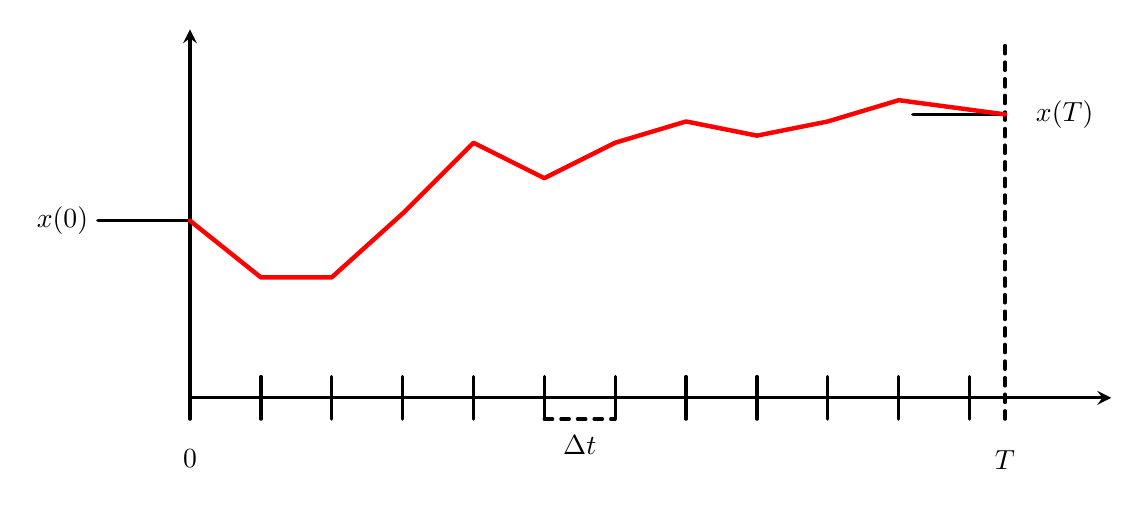
\begin{tikzpicture}[
        scale=0.9,
        >=stealth,
        line cap=round,
        line join=round
    ]
    % TODO: should add initial conditions of each interval to show setup explicitly
        % axes
        \draw[very thick,->] (0,-.3) -- (0,5.2);
        \draw[very thick,->] (0,0)     -- (13,0);

        % time ticks
        \foreach \x in {1,...,11}{
        \draw[very thick] (\x,0.3) -- (\x,-0.3);
        }

        % dashed line at T
        \draw[very thick,dashed] (11.5,-.3) -- (11.5,5.0);

        % horizontal levels x(0) and x(T)
        \draw[very thick] (-1.3,2.5) -- (0,2.5);      % x(0)
        \draw[very thick] (10.2,4.0) -- (11.5,4.0);   % x(T)

        % sample path
        \draw[ultra thick,red]
        (0,2.5)  --
        (1,1.7)  --
        (2,1.7)  --
        (3,2.6)  --
        (4,3.6)  --
        (5,3.1)  --
        (6,3.6)  --
        (7,3.9)  --
        (8,3.7)  --
        (9,3.9)  --
        (10,4.2) --
        (11.5,4.0);

        \draw[very thick,dashed] (5,-0.3) -- (6,-0.3);

        \node[below] at (0,-.6) {$0$};
        \node[below] at (11.5,-.6) {$T$};
        \node[below] at (5.5,-.4) {$\Delta t$};

        \node[left]  at (-1.3,2.5) {$x(0)$};
        \node[right] at (11.8,4.0) {$x(T)$};

    \end{tikzpicture}
    \caption{Schematic of the multiple shooting method. The long interval $[0,T]$ is partitioned into $M$ sub-intervals $[t_i,t_{i+1}]$ with $t_i = i\Delta t$. On each sub-interval, a local trajectory $\mathbf{x}_i(t)$ is integrated from an independent initial value $\mathbf{c}_i \approx \mathbf{x}(t_i)$. Continuity constraints enforce that the end point of one segment matches the initial value of the next, $\mathbf{x}_i(t_{i+1}) = \mathbf{c}_{i+1}$, so that the segments form a single continuous solution of the BVP. Note that the solution is not necessarily piecewise linear (it just is for the case shown here).}
    \label{fig:multiple_shooting_diagram}
\end{figure}

\subsection{The Finite Difference Method}

We can arrive at a powerful alternative to shooting methods by taking the concept of multiple shooting to its logical limit. Recall that in multiple shooting, we divided the domain $[0, T]$ into $M$ sub-intervals and solved an IVP over each small segment $[t_i, t_{i+1}]$. We then glued these solutions together by enforcing continuity $\mathbf{x}(t_{i+1}; \mathbf{c}_i) = \mathbf{c}_{i+1}$. Now, imagine we decrease the interval size $\Delta t$ until it is so small that a single step of the simplest explicit Euler method is sufficiently accurate to represent the ODE dynamics. In this limit, the condition that the solution at the end of interval $i$ matches the start of interval $i+1$ becomes a simple algebraic relationship:
\begin{equation}
    \mathbf{c}_{i+1} = \mathbf{c}_i + \Delta t \, \mathbf{f}(\mathbf{c}_i, t_i)
\end{equation}
This equation relates the values of the solution at adjacent grid points directly without needing to run an ODE solver. If we rearrange this, we see that it effectively approximates the derivative using the slope between points. This viewpoint is what motivates finite differences. Instead of integrating the differential equation, we discretize the differential operator itself. We replace the continuous domain with a discrete grid of $M+1$ points (nodes) and replace the derivatives in the differential equation with algebraic difference quotients involving the values at these nodes. This converts the BVP into a large system of coupled nonlinear algebraic equations, which we can solve using Newton's method.

\begin{figure}[H]
    \centering
    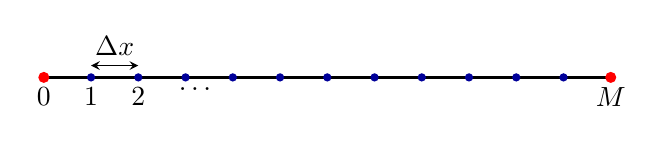
\begin{tikzpicture}[>=stealth]

    % parameters
    \def\M{12}        % number of intervals
    \def\dx{0.6}      % spacing between grid points

    % horizontal line
    \draw[thick] (0,0) -- (\M*\dx,0);

    % interior grid points (blue)
    \foreach \k in {1,...,\numexpr\M-1\relax}{
    \fill[blue!60!black] (\k*\dx,0) circle (1.5pt);
    }

    % boundary grid points (red)
    \fill[red] (0,0) circle (2pt);
    \fill[red] (\M*\dx,0) circle (2pt);

    % labels x=0 and x=1
    % \node[above] at (0,0.05) {$x=0$};
    % \node[above] at (\M*\dx,0.05) {$x=1$};

    % index labels
    \node[below] at (0,0) {$0$};
    \node[below] at (\dx,0) {$1$};
    \node[below] at (2*\dx,0) {$2$};
    \node[below] at (3.2*\dx,0) {$\dots$};
    \node[below] at (\M*\dx,0) {$M$};

    % Delta x arrow
    \draw[<->] (\dx,0.15) -- (2*\dx,0.15);
    \node[above] at (1.5*\dx,0.15) {$\Delta x$};

    \end{tikzpicture}
    \caption{Discretization of the domain into $M$ intervals of width $\Delta x$.}
    \label{fig:finite_difference_diagram}
\end{figure}


\paragraph*{Finite Difference Approximations}

To formalize this, we define a grid $x_m = x_0 + m\Delta x$ for $m=0, 1, \dots, M$, where $\Delta x$ is the grid spacing. We seek approximate values $C_m \approx c(x_m)$. We approximate the derivatives $f^{(p)}(x)$ at a node using a weighted sum of function values at neighboring nodes:
\begin{equation}
    f^{(p)}(x_0) \approx \frac{1}{(\Delta x)^p} \sum_{m} \alpha_m f(x_m)
\end{equation}
We can derive these coefficients $\alpha_m$ and analyze their accuracy using Taylor series expansions. For the first derivative $f'(x)$, a symmetric \textbf{central difference} uses the points immediately to the left and right:
\begin{equation}
    f'(x) \approx \frac{f(x + \Delta x) - f(x - \Delta x)}{2\Delta x}
\end{equation}
By expanding $f(x+\Delta x)$ and $f(x-\Delta x)$ in Taylor series up to the third order and subtracting them, terms involving $f(x)$ and $f''(x)$ cancel out, leaving the first derivative term plus an error term proportional to $(\Delta x)^2 f'''(x)$. Thus, this approximation is \textit{second-order accurate}, or $O(\Delta x^2)$.

For the second derivative $f''(x)$, which appears frequently in diffusion and wave problems, we combine the values at $x-\Delta x$, $x$, and $x+\Delta x$:
\begin{equation}
    f''(x) \approx \frac{f(x - \Delta x) - 2f(x) + f(x + \Delta x)}{(\Delta x)^2}
\end{equation}
Again, Taylor analysis confirms this approximation is second-order accurate. Specifically, the error term scales with $(\Delta x)^2 f^{(4)}(x)$. High-order accuracy is desirable because it implies that refining the grid (reducing $\Delta x$) leads to a rapid reduction in numerical error.

\paragraph*{Application: Reaction-Diffusion System}

Let us apply this method to the concrete physical example of a steady-state reaction-diffusion system in a 1D slab. The governing equation is
\begin{equation}
    \frac{d^2 c}{dx^2} = -r(c)
\end{equation}
where $c(x)$ is the concentration and $r(c)$ is the reaction rate. The domain is $x \in [0, 1]$. We impose generalized Robin boundary conditions at both ends, which relate the concentration and its flux:
\begin{align}
    x=0: & \quad A_0 \frac{dc}{dx} + B_0 c = C_0 \\
    x=1: & \quad A_1 \frac{dc}{dx} + B_1 c = C_1
\end{align}
We discretize the domain into $M$ intervals of size $\Delta x = 1/M$, creating $M+1$ unknown variables $c_0, c_1, \dots, c_M$. For every interior node $m = 1, \dots, M-1$, we replace the second derivative with the central difference approximation derived above. Substituting this into the ODE produces one algebraic equation per node:
\begin{equation}
    \frac{1}{(\Delta x)^2} (c_{m-1} - 2c_m + c_{m+1}) + r(c_m) = 0
\end{equation}
This provides $M-1$ equations for our $M+1$ unknowns. To close the system, we must derive equations for the two boundary nodes $m=0$ and $m=M$ using the boundary conditions. The boundary conditions involve the first derivative $dc/dx$. We must approximate this derivative using the available grid points. At the left boundary ($x=0$, node $m=0$), we cannot use a central difference because there is no node at $x_{-1}$. Instead, we can use a forward difference. A simple first-order forward difference is $(c_1 - c_0)/\Delta x$. However, since our interior scheme is second-order accurate ($O(\Delta x^2)$), using a first-order boundary approximation ($O(\Delta x)$) would degrade the global accuracy of the solution. To maintain second-order accuracy, we employ a three-point forward difference approximation for the derivative at the boundary. The boundary equation at $x=0$ becomes
\begin{equation}
    g_0(\mathbf{c}) = A_0 \left[ \frac{-3c_0 + 4c_1 - c_2}{2\Delta x} \right] + B_0 c_0 - C_0 = 0
\end{equation}
Similarly, at the right boundary ($x=1$, node $m=M$), we use a three-point backward difference:
\begin{equation}
    g_M(\mathbf{c}) = A_1 \left[ \frac{3c_M - 4c_{M-1} + c_{M-2}}{2\Delta x} \right] + B_1 c_M - C_1 = 0
\end{equation}
(Note: these three-point formulas require $M \ge 2$ so that the necessary interior points exist.) Collecting the equations for the boundaries and the interior points, we obtain a system of $M+1$ nonlinear algebraic equations for the $M+1$ unknowns. We define the residual vector function $\mathbf{G}(\mathbf{c}) = \mathbf{0}$, where
\begin{equation}
    \mathbf{G}(\mathbf{c}) = \begin{bmatrix}
        g_0(\mathbf{c}) \\
        \frac{1}{(\Delta x)^2} (c_0 - 2c_1 + c_2) + r(c_1) \\
        \vdots \\
        \frac{1}{(\Delta x)^2} (c_{M-2} - 2c_{M-1} + c_M) + r(c_{M-1}) \\
        g_M(\mathbf{c})
    \end{bmatrix} = \mathbf{0}
\end{equation}
This system is usually sparse and structured (tridiagonal or pentadiagonal), which makes it computationally efficient to solve using Newton-Raphson methods, such as \texttt{fsolve} in MATLAB or \texttt{scipy.optimize.root} in Python.

\begin{figure}[H]
    \centering
    \includegraphics[width=0.95\textwidth]{figs/ode/finite_difference_convergence.pdf}
    \caption{Finite difference solution and convergence analysis. Left: Numerical solutions for the reaction-diffusion problem ($c'' = -kc$ with boundary conditions $c(0)=1, c(1)=0$) using varying grid resolutions ($M=10, 20, 40$) compared to the exact analytical solution (solid gray line). Right: Log-log convergence plot showing the maximum error between the numerical and exact solutions versus the grid spacing $\Delta x$. The error data points (black dots) align almost perfectly with the red dashed reference line representing quadratic scaling, which confirms the theoretical $O(\Delta x^2)$ accuracy of the central difference scheme.}
    \label{fig:fd_convergence}
\end{figure}

The accuracy of the numerical solution depends heavily on the grid spacing. As shown in \autoref{fig:fd_convergence}, a plot of the error against the grid spacing $\Delta x$ on a logarithmic scale has a slope of 2. This empirically verifies that our choice of central differences for the interior and three-point differences for the boundaries gives a globally second-order accurate solution. While the finite difference method requires solving a large simultaneous system (unlike the shooting method, which solves small IVPs sequentially), it is generally more robust and less sensitive to initial guesses, particularly for stiff or unstable differential equations.

\paragraph*{Accuracy Analysis of Finite Differences}

To justify the accuracy of the finite difference approximations used in the previous section, we use Taylor's theorem. This allows us to quantify the local truncation error introduced by discretizing the continuous differential operator. Consider the central difference approximation for the first derivative. We expand the function values at the neighboring nodes $x + \Delta x$ and $x - \Delta x$ around the central point $x$:
\begin{align}
    f(x + \Delta x) &= f(x) + \Delta x f'(x) + \frac{(\Delta x)^2}{2} f''(x) + \frac{(\Delta x)^3}{6} f'''(x) + O(\Delta x^4) \\
    f(x - \Delta x) &= f(x) - \Delta x f'(x) + \frac{(\Delta x)^2}{2} f''(x) - \frac{(\Delta x)^3}{6} f'''(x) + O(\Delta x^4)
\end{align}
Subtracting the second equation from the first causes the even-order derivative terms to cancel out. We are left with the difference $f(x + \Delta x) - f(x - \Delta x) = 2\Delta x f'(x) + \frac{(\Delta x)^3}{3} f'''(x) + \dots$. Dividing by $2\Delta x$ isolates the first derivative:
\begin{equation}
    \frac{f(x + \Delta x) - f(x - \Delta x)}{2\Delta x} = f'(x) + \frac{(\Delta x)^2}{6} f'''(x) + \dots
\end{equation}
The dominant error term is proportional to $(\Delta x)^2$. Consequently, we say this approximation is second-order accurate, or $O(\Delta x^2)$. A similar procedure for the second derivative approximation $f''(x) \approx (f(x+\Delta x) - 2f(x) + f(x-\Delta x))/(\Delta x)^2$ also yields an error term proportional to $(\Delta x)^2 f^{(4)}(x)$, confirming that the standard central difference scheme maintains second-order consistency throughout the domain.

\paragraph*{Relation to Multiple Shooting}

We've mentioned this before, but it is instructive to recognize that the finite difference method is not entirely distinct from the shooting methods discussed earlier; rather, it is a limiting case. Recall that in the multiple shooting method, we partition the domain $[0, T]$ into $M$ sub-intervals and solve an IVP on each segment, enforcing continuity $\mathbf{c}_{i} = \mathbf{x}(t_i; \mathbf{c}_{i-1})$ at the nodes. If we decrease the interval size $\Delta t$ until it is small enough that a single step of an explicit Euler integrator is sufficient, the continuity condition simplifies. The integration step becomes $\mathbf{c}_i = \mathbf{c}_{i-1} + \Delta t \, \mathbf{f}(\mathbf{c}_{i-1}, t_{i-1})$. Rearranging this yields $(\mathbf{c}_i - \mathbf{c}_{i-1})/\Delta t = \mathbf{f}(\mathbf{c}_{i-1})$, which is exactly the finite difference formulation using a forward difference. Thus, we can view the finite difference method as a multiple shooting method where the number of intervals $M$ approaches the number of grid points, and the ``shooting'' (IVP integration) is replaced by a simple algebraic step. The resulting system of nonlinear equations involves $(M+1)N$ variables and equations, which can be solved simultaneously using Newton-Raphson.

\subsection{Basis Function Expansions}

Basis function expansion methods (also called spectral methods or weighted residual methods) take a different approach than the grid-discretization methods discussed above. We approximate the solution $c(x)$ as a continuous function constructed from a linear combination of pre-selected basis functions $\{\Phi_j(x)\}_{j=1}^M$. The approximate solution is written as
\begin{equation}
    c(x) \approx \sum_{j=1}^M c_j \Phi_j(x)
\end{equation}
The problem of solving the differential equation is thus transformed into the problem of finding the optimal set of scalar coefficients $c_1, \dots, c_M$. This approach is powerful because, with a wise choice of basis functions (such as orthogonal polynomials or Fourier modes), we can achieve high accuracy with relatively few coefficients.

\paragraph*{Handling Boundary Conditions}

Before determining the coefficients, we must ensure the boundary conditions are satisfied. Consider a general BVP with Dirichlet boundary conditions:
\begin{equation}
    \frac{d^2c}{dx^2} = f(x), \quad c(0) = a, \quad c(1) = b
    \label{eq:bvp-dirichlet}
\end{equation}
If our basis functions are arbitrary, satisfying $c(0)=a$ and $c(1)=b$ constrains the coefficients $c_j$ in a complicated way. To simplify this, we use a splitting technique. We assume the solution can be decomposed into a particular function $c_p(x)$ and a homogeneous function $c_h(x)$:
\begin{equation}
    c(x) = c_p(x) + c_h(x)
\end{equation}
The particular function $c_p(x)$ is chosen solely to satisfy the boundary conditions. For instance, the linear function $c_p(x) = a + (b-a)x$ satisfies $c_p(0)=a$ and $c_p(1)=b$. The remaining part, $c_h(x)$, must then satisfy homogeneous boundary conditions ($c_h(0)=0, c_h(1)=0$) so that the sum matches the original BCs. By substituting this decomposition into the original ODE, we get a new differential equation for $c_h(x)$ where the forcing term is modified by derivatives of $c_p(x)$ but the boundary conditions are strictly zero. Without loss of generality, we can therefore restrict our study to BVPs with homogeneous boundary conditions. We choose basis functions $\{\Phi_j(x)\}$ that individually satisfy $\Phi_j(0) = 0$ and $\Phi_j(1) = 0$. Consequently, any linear combination of these functions automatically satisfies the boundary conditions, allowing us to focus entirely on satisfying the differential equation inside the domain.

\paragraph*{Weighted Residuals}

We substitute our expansion $c(x) = \sum c_j \Phi_j(x)$ into the differential equation $c'' - f(x) = 0$ (\autoref{eq:bvp-dirichlet}). Since our approximation is not exact, this substitution produces a non-zero residual function $R(x; \mathbf{c})$:
\begin{equation}
    R(x; \mathbf{c}) = \sum_{j=1}^M c_j \Phi_j''(x) - f(x) \neq 0
\end{equation}
We cannot force the residual to be zero everywhere (that would require the exact solution). Instead, we enforce that the residual is zero in a weighted average sense. We introduce a set of test functions (or weight functions) $\{\Psi_i(x)\}_{i=1}^M$ and require the integral of the residual against each test function to vanish:
\begin{equation}
    \int_0^1 \Psi_i(x) R(x; \mathbf{c}) \, dx = 0, \quad \text{for } i = 1, \dots, M
\end{equation}
Expanding this integral, we get a system of linear equations for the coefficients $c_j$:
\begin{equation}
    \sum_{j=1}^M c_j \left( \int_0^1 \Psi_i(x) \Phi_j''(x) \, dx \right) = \int_0^1 \Psi_i(x) f(x) \, dx
\end{equation}
This can be written as a matrix system $\mathbf{A}\mathbf{c} = \mathbf{b}$. The choice of the test functions $\{\Psi_i(x)\}$ determines the specific numerical method. Two such choices are the collocation method and the Galerkin method.

\paragraph*{The Collocation Method}

In the collocation method, we choose the test functions to be Dirac delta functions centered at specific points $x_i$: $\Psi_i(x) = \delta(x - x_i)$. The integral property of the delta function sifts out the value of the residual at $x_i$. Physically, this implies we are forcing the differential equation to hold exactly at a set of $M$ discrete collocation points $\{x_i\}_{i=1}^M$. The equations become
\begin{equation}
    \sum_{j=1}^M c_j \Phi_j''(x_i) = f(x_i), \quad \text{for } i = 1, \dots, M
\end{equation}
Usually, the collocation points are chosen to be the roots of orthogonal polynomials (such as Legendre polynomials) to minimize the error between points, a technique known as orthogonal collocation.

\paragraph*{The Galerkin Method}

In the Galerkin method, we choose the test functions to be the same as the basis functions: $\Psi_i(x) = \Phi_i(x)$. We are basically projecting the residual onto the space spanned by the basis functions and demanding that the error is orthogonal to our approximation space. The condition is
\begin{equation}
    \sum_{j=1}^M c_j \left( \int_0^1 \Phi_i(x) \Phi_j''(x) \, dx \right) = \int_0^1 \Phi_i(x) f(x) \, dx
\end{equation}
If the basis functions $\{\Phi_j(x)\}$ are eigenfunctions of the differential operator (e.g., $\Phi_j'' = \lambda_j \Phi_j$) and are orthogonal (meaning $\int \Phi_i \Phi_j dx = 0$ for $i \neq j$), the matrix on the left-hand side becomes diagonal or highly structured, making the system trivial to solve.

\begin{exampleBox}
    \textbf{Example: Solving a BVP with Basis Functions}
    
    Consider the following BVP:
    \begin{equation}
        \frac{d^2c}{dx^2} - c = \exp(-x^2), \quad c(0) = c(1) = 0
    \end{equation}
    Since the boundary conditions are homogeneous and Dirichlet, a natural choice for basis functions are the sine modes, which are eigenfunctions of the second derivative operator:
    \begin{equation}
        \Phi_j(x) = \sin(j \pi x), \quad j=1, \dots, M
    \end{equation}
    These functions satisfy $\Phi_j(0)=\Phi_j(1)=0$ automatically. We seek $c(x) = \sum c_j \sin(j \pi x)$.
    
    \textbf{1. Collocation Approach:}
    We choose $M$ points $x_i$ evenly spaced in $(0, 1)$. We substitute the sum into the ODE ($c'' - c$) and evaluate at each $x_i$:
    \begin{equation}
        \sum_{j=1}^M c_j \left[ -(j\pi)^2 \sin(j\pi x_i) - \sin(j\pi x_i) \right] = \exp(-x_i^2)
    \end{equation}
    This is a linear system $\mathbf{A}\mathbf{c} = \mathbf{b}$ where $A_{ij} = -((j\pi)^2 + 1)\sin(j\pi x_i)$.
    
    \textbf{2. Galerkin Approach:}
    We multiply the residual by $\Phi_i(x) = \sin(i \pi x)$ and integrate from 0 to 1. Due to the orthogonality of sines, the cross terms in the sum vanish ($\int \sin(i\pi x)\sin(j\pi x) dx = 0$ for $i \neq j$). The term involving the second derivative becomes:
    \begin{equation}
        \int_0^1 \sin(i \pi x) \frac{d^2}{dx^2} \left( c_i \sin(i \pi x) \right) dx = -c_i (i\pi)^2 \int_0^1 \sin^2(i \pi x) dx = -c_i \frac{(i\pi)^2}{2}
    \end{equation}
    Similarly, the term $\int c \Phi_i dx$ yields $c_i/2$. The equation for coefficient $c_i$ decouples completely:
    \begin{equation}
        -\frac{1}{2} \left[ (i\pi)^2 + 1 \right] c_i = \int_0^1 \exp(-x^2) \sin(i \pi x) dx
    \end{equation}
    We can calculate the integral on the right-hand side (numerically or analytically) and directly divide by the scalar factor $-\frac{1}{2}[(i\pi)^2 + 1]$ to find each $c_i$.
    
    \begin{figure}[H]
        \centering
        \includegraphics[width=0.6\textwidth]{figs/ode/bvp_coll_galerkin.pdf}
        \caption{Comparison of collocation and Galerkin methods for the example BVP. As the number of basis functions $N$ increases (colored lines), both methods converge to the true solution (gray band). The Galerkin method minimizes the global integrated error, while collocation drives the error to zero specifically at the chosen points.}
        \label{fig:bvp_coll_galerkin}
    \end{figure}
\end{exampleBox}

\subsection{The Finite Element Method}

The basis function expansion methods discussed previously, particularly when using global polynomials or eigenfunctions (like sine waves), have a significant computational issue. This issue is that these functions are global; that is, they are non-zero over the entire domain. Consequently, when we compute the inner products for the Galerkin method, every basis function interacts with every other basis function. This results in a dense system matrix $\mathbf{A}$, where every entry is potentially non-zero. Solving a dense linear system requires $O(M^3)$ operations, which becomes prohibitively expensive as the number of modes $M$ increases. Furthermore, finding suitable global basis functions for complex, irregular geometries is often impossible.

To overcome these limitations, we introduce the \textbf{finite element method (FEM)}. The philosophy of FEM is to retain the integral formulation of the Galerkin method but to replace the global basis functions with \textit{local} basis functions.

\paragraph*{Local Basis Functions}

We partition the domain $[0, 1]$ into a grid of nodes $x_0, x_1, \dots, x_M$, similar to the finite difference grid. However, instead of approximating the derivative at a point, we define basis functions $\Phi_m(x)$ that are non-zero only over a small sub-interval around node $x_m$. The simplest choice is the piecewise linear ``hat'' or ``tent'' function defined as:
\begin{equation}
    \Phi_m(x) = \begin{cases} 
      \frac{x - x_{m-1}}{\Delta x} & x_{m-1} < x \le x_m \\
      \frac{x_{m+1} - x}{\Delta x} & x_m < x < x_{m+1} \\
      0 & \text{otherwise} 
   \end{cases}
\end{equation}
where $\Delta x$ is the spacing between nodes. Each function $\Phi_m(x)$ rises linearly from 0 to 1 and falls back to 0 over a span of $2\Delta x$. Taking linear combinations of these local tent functions allows us to construct a global piecewise-linear approximation of any given function. Importantly, $\Phi_i(x)$ and $\Phi_j(x)$ have no overlap if $|i - j| > 1$. This locality property guarantees that the vast majority of integrals in the Galerkin formulation will be zero, leading to a sparse, banded matrix that is computationally efficient to solve.

\begin{figure}[H]
    \centering
    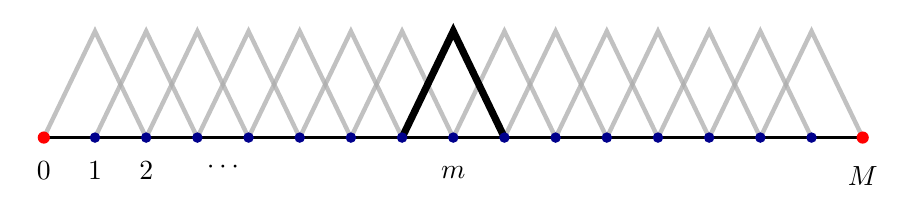
\begin{tikzpicture}[x=0.65cm,y=1cm]
    % parameters
    \def\M{16}   % right endpoint index (labeled M)
    \def\m{8}    % highlighted index (labeled m)
    \def\H{1.35} % hat height

    \pgfmathtruncatemacro{\Mminusone}{\M-1}

    % baseline
    \draw[line width=1.2pt] (0,0) -- (\M,0);

    % grey hat functions (all i = 1,...,M-1)
    \foreach \i in {1,...,\Mminusone}{
        \draw[gray!65,opacity=0.75,line width=1.6pt,line cap=round]
        ({\i-1},0) -- (\i,\H) -- ({\i+1},0);
    }

    % highlighted hat at i = m
    \draw[black,line width=2.6pt,line cap=round]
        ({\m-1},0) -- (\m,\H) -- ({\m+1},0);

    % nodes on the line
    \fill[red] (0,0) circle (2.2pt);
    \fill[red] (\M,0) circle (2.2pt);
    \foreach \i in {1,...,\Mminusone}{
        \fill[blue!55!black] (\i,0) circle (1.9pt);
    }

    % labels
    % \node[left=10pt]  at (0,0)  {$x=0$};
    % \node[right=10pt] at (\M,0) {$x=1$};

    \node[below=5pt] at (0,0) {$0$};
    \node[below=5pt] at (1,0) {$1$};
    \node[below=5pt] at (2,0) {$2$};
    \node[below=5pt] at (3.5,0) {$\cdots$};
    \node[below=7pt] at (\m,0) {$m$};
    \node[below=7pt] at (\M,0) {$M$};
    \end{tikzpicture}
    \caption{Local tent basis functions for the FEM.}
    \label{fig:fem_basis}
\end{figure}

\paragraph*{The Weak Formulation}

Let us apply this to our model problem:
\begin{equation}
    \frac{d^2c}{dx^2} - c = \exp(-x^2), \quad c(0)=0, \quad c(1)=0
\end{equation}
We approximate the solution as a linear combination of these tent functions: $c(x) \approx \sum_{j=1}^{M-1} c_j \Phi_j(x)$. Note that we exclude $j=0$ and $j=M$ from the unknowns because the boundary conditions $c(0)=0$ and $c(1)=0$ fix those coefficients to zero. We now plug this appoximation into the Galerkin condition. If we tried to do this in the ``strong'' form, i.e.,
\begin{equation}
    \int_0^1 \bigl(c_h''(x) - c_h(x) - f(x)\bigr)\,\Phi_i(x)\,dx = 0
\end{equation}
we immediately run into the issue that since $\Phi_j$ is only piecewise linear, $\Phi_j'$ is piecewise constant and $\Phi_j''$ is not an ordinary function at all (it lives at the nodes as delta spikes). Considering this, the standard FEM trick is to integrate by parts once so that we only need first derivatives. Concretely,
\begin{equation}
    \int_0^1 c_h''(x)\,\Phi_i(x)\,dx
    = \Bigl[c_h'(x)\,\Phi_i(x)\Bigr]_{0}^{1} - \int_0^1 c_h'(x)\,\Phi_i'(x)\,dx
\end{equation}
For interior test functions $i=1,\dots,M-1$, the hats satisfy $\Phi_i(0)=\Phi_i(1)=0$, so the boundary term drops:
\begin{equation}
    \Bigl[c_h'(x)\,\Phi_i(x)\Bigr]_{0}^{1} = 0
\end{equation}
So the weak (integrated-by-parts) Galerkin equations become
\begin{equation}
    -\int_0^1 c_h'(x)\,\Phi_i'(x)\,dx - \int_0^1 c_h(x)\,\Phi_i(x)\,dx
    = \int_0^1 f(x)\,\Phi_i(x)\,dx
    \qquad i=1,\dots,M-1
\end{equation}
where here $f(x)=e^{-x^2}$. Now, we substitute the expansion $c_h=\sum_{j=1}^{M-1}c_j\Phi_j$ and pull the coefficients $c_j$ outside the integrals:
\begin{equation}
    \sum_{j=1}^{M-1} c_j\left(
        -\int_0^1 \Phi_j'(x)\,\Phi_i'(x)\,dx
        -
        \int_0^1 \Phi_j(x)\,\Phi_i(x)\,dx
    \right)
    = \int_0^1 f(x)\,\Phi_i(x)\,dx
\end{equation}
At this point, it is helpful to name the two standard FEM matrices. The derivative term is the \emph{stiffness} matrix,
\begin{equation}
    K_{ij} = \int_0^1 \Phi_j'(x)\,\Phi_i'(x)\,dx
\end{equation}
and the term with the functions themselves is the \emph{mass} matrix,
\begin{equation}
    M_{ij} = \int_0^1 \Phi_j(x)\,\Phi_i(x)\,dx
\end{equation}
The right-hand side is just the load vector entry
\begin{equation}
    b_i = \int_0^1 f(x)\,\Phi_i(x)\,dx
\end{equation}
With this notation, the linear system is simply
\begin{equation}
    \sum_{j=1}^{M-1}\bigl(-K_{ij}-M_{ij}\bigr)c_j = b_i
    \qquad i=1,\dots,M-1,
\end{equation}
or, in matrix form, $\mathbf{A}\mathbf{c}=\mathbf{b}$ with $A_{ij}=-K_{ij}-M_{ij}$. (Note that since our operator is formally $d^2/dx^2 - I$, which is negative definite, the matrix $\mathbf{A}$ is negative definite. In many texts, the problem is multiplied by $-1$ to yield a positive-definite system $(K+M)\mathbf{c} = -\mathbf{b}$. Just be aware of this.) The big practical win here is sparsity: each hat $\Phi_i$ only overlaps with $\Phi_{i-1}$ and $\Phi_{i+1}$, so
\begin{equation}
    K_{ij}=M_{ij}=0\qquad\text{whenever}\qquad |i-j|>1
\end{equation}
meaning $\mathbf{A}$ is tridiagonal. On a uniform grid with spacing $\Delta x$, the stiffness entries come straight from the fact that $\Phi_i'$ is $\frac{1}{\Delta x}$ on the left element and $-\frac{1}{\Delta x}$ on the right element. For the diagonal,
\begin{equation}
    K_{ii}
    = \int_{x_{i-1}}^{x_i}\left(\frac{1}{\Delta x}\right)^2 dx
      + \int_{x_i}^{x_{i+1}}\left(-\frac{1}{\Delta x}\right)^2 dx
    = \frac{2}{\Delta x}
\end{equation}
and for the neighbors (say $i$ and $i+1$), the derivatives have opposite signs on the shared element $[x_i,x_{i+1}]$, giving
\begin{equation}
    K_{i,i+1}
    = \int_{x_i}^{x_{i+1}}\left(-\frac{1}{\Delta x}\right)\left(\frac{1}{\Delta x}\right)\,dx
    = -\frac{1}{\Delta x}
\end{equation}
and similarly $K_{i,i-1}=-\frac{1}{\Delta x}$. For the mass matrix, you can either do the little triangles-by-hand integrals or just remember the standard results for linear elements. The diagonal is
\begin{equation}
    M_{ii} = \int_0^1 \Phi_i(x)^2\,dx = \frac{2}{3}\Delta x,
\end{equation}
and the off-diagonal neighbor coupling is
\begin{equation}
    M_{i,i+1} = \int_0^1 \Phi_i(x)\,\Phi_{i+1}(x)\,dx = \frac{1}{6}\Delta x
\end{equation}
with the same value for $M_{i,i-1}$. Putting these together, the $i$th row of the FEM system (only involving $c_{i-1},c_i,c_{i+1}$) reads
\begin{equation}
    -\Bigl(K_{i,i-1}c_{i-1}+K_{ii}c_i+K_{i,i+1}c_{i+1}\Bigr)
    -\Bigl(M_{i,i-1}c_{i-1}+M_{ii}c_i+M_{i,i+1}c_{i+1}\Bigr)
    = b_i,
\end{equation}
i.e.,
\begin{equation}
    -\left(-\frac{1}{\Delta x}c_{i-1} + \frac{2}{\Delta x}c_i - \frac{1}{\Delta x}c_{i+1}\right)
    -\left(\frac{\Delta x}{6}c_{i-1} + \frac{2\Delta x}{3}c_i + \frac{\Delta x}{6}c_{i+1}\right)
    = \int_0^1 e^{-x^2}\,\Phi_i(x)\,dx
\end{equation}
If we group the terms in the nicer ``stencil'' form, we get
\begin{equation}
    \frac{1}{\Delta x}\bigl(c_{i-1}-2c_i+c_{i+1}\bigr)
    -
    \frac{\Delta x}{6}\bigl(c_{i-1}+4c_i+c_{i+1}\bigr)
    =
    \int_0^1 e^{-x^2}\,\Phi_i(x)\,dx
\end{equation}
This system is tridiagonal and sparse, so we have solved the computational efficiency problem of global basis functions. Interestingly, if we inspect the first term, we see it matches the standard central difference approximation multiplied by $\Delta x$. However, the FEM formulation also has a mass matrix term (the second group) which averages the reaction term over neighboring nodes (this causes higher accuracy for certain problem classes).

\begin{figure}[H]
    \centering
    \includegraphics[width=0.6\textwidth]{figs/ode/fem_convergence.pdf}
    \caption{Finite element method solution to $c'' - c = \exp(-x^2)$. Using piecewise linear tent basis functions, the solution converges rapidly. Even with a small number of elements ($N=3, 4, 7$), the method captures the curvature of the solution effectively.}
    \label{fig:fem_convergence}
\end{figure}

The finite element method thus combines the best of both worlds: (1) the geometric flexibility and sparse matrix structure of finite differences, and (2) the error minimization and integral formulation of weighted residual methods.

\subsection{The Finite Volume Method}

FEM is very clean mathematically (same functions for both the expansion and the testing), but in a lot of transport problems, we really want to build conservation in by construction. That is the motivating idea behind the finite volume method: instead of asking for the residual to be orthogonal to the same tent functions, we ask for the residual to have zero \emph{average} over a little control volume around each node. You can still think of this as a Galerkin/weighted-residual method, but with a different set of test functions, the \textit{conjugate basis functions}. To be explicit, we keep the same piecewise-linear approximation for the solution using the tent functions $\{\Phi_i\}_{i=1}^{M-1}$,
\begin{equation}
    c(x) \approx \sum_{j=1}^{M-1} c_j \Phi_j(x)
\end{equation}
so $c(x)$ is continuous and varies linearly between nodes. The change is the test function. For each interior node $x_i=i\Delta x$, we associate a control volume that extends halfway to the neighboring nodes; it is convenient to denote its faces by
\begin{equation}
    x_{i-1/2} = x_i - \frac{\Delta x}{2},
    \qquad
    x_{i+1/2} = x_i + \frac{\Delta x}{2}
\end{equation}
The conjugate basis function $\Psi_i$ is just a normalized top-hat on that control volume (so integrals become averages):
\begin{equation}
    \Psi_i(x) =
    \begin{cases}
        \dfrac{1}{\Delta x}, & (i-\tfrac{1}{2})\Delta x < x < (i+\tfrac{1}{2})\Delta x,\\[10pt]
        0, & \text{otherwise}
    \end{cases}
\end{equation}

\begin{figure}[H]
    \centering
    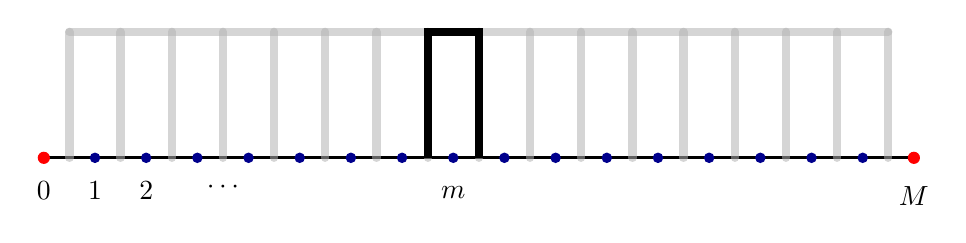
\begin{tikzpicture}[x=0.65cm,y=1cm]
        % parameters
        \def\M{17}    % right endpoint index (labeled M)
        \def\m{8}     % highlighted cell index (labeled m)
        \def\H{1.6}   % height

        \pgfmathtruncatemacro{\MMone}{\M-1}

        % baseline
        \draw[line width=1.2pt] (0,0) -- (\M,0);

        % background "box" grid: verticals at half-integers + top bar
        \draw[gray!60,opacity=0.55,line width=3.0pt,line cap=round]
        (0.5,\H) -- ({\M-0.5},\H);

        \foreach \k in {0,...,\MMone}{
        \draw[gray!60,opacity=0.55,line width=3.0pt,line cap=round]
            ({\k+0.5},0) -- ({\k+0.5},\H);
        }

        % highlighted box over cell m : [m-1/2, m+1/2]
        \draw[line width=2.8pt, line join=miter] ({\m-0.5},0) -- ({\m-0.5},\H) -- ({\m+0.5},\H) -- ({\m+0.5},0);

        % nodes on the line
        \fill[red] (0,0) circle (2.2pt);
        \fill[red] (\M,0) circle (2.2pt);
        \foreach \i in {1,...,\MMone}{
        \fill[blue!55!black] (\i,0) circle (1.9pt);
        }

        % labels
        \node[below=5pt] at (0,0) {$0$};
        \node[below=5pt] at (1,0) {$1$};
        \node[below=5pt] at (2,0) {$2$};
        \node[below=5pt] at (3.5,0) {$\cdots$};
        \node[below=7pt] at (\m,0) {$m$};
        \node[below=7pt] at (\M,0) {$M$};
    \end{tikzpicture}
    \caption{Finite volume method conjugate basis functions (control volumes).}
    \label{fig:fvm_conjugate_basis_functions}
\end{figure}

Now, we apply this to our model problem
\begin{equation}
    \frac{d^2 c}{dx^2} - c = \exp(-x^2), \qquad c(0)=c(1)=0
\end{equation}
The weighted residual statement with the conjugate test function is
\begin{equation}
    \int_0^1 \left[\frac{d^2 c}{dx^2} - c\right]\Psi_i(x)\,dx
    =
    \int_0^1 \exp(-x^2)\,\Psi_i(x)\,dx,
    \qquad i=1,2,\dots,M-1
\end{equation}
and because $\Psi_i$ is only nonzero on the control volume, this is just the local averaged balance
\begin{equation}
    \frac{1}{\Delta x}\int_{x_{i-1/2}}^{x_{i+1/2}}
    \left[\frac{d^2 c}{dx^2} - c\right]\,dx
    =
    \frac{1}{\Delta x}\int_{x_{i-1/2}}^{x_{i+1/2}} \exp(-x^2)\,dx
\end{equation}
The second derivative term turns into a clean flux difference automatically (this is the conservation-law flavor showing up). Using the fundamental theorem of calculus,
\begin{equation}
    \frac{1}{\Delta x}\int_{x_{i-1/2}}^{x_{i+1/2}} \frac{d^2 c}{dx^2}\,dx
    =
    \frac{1}{\Delta x}\left[\left.\frac{dc}{dx}\right|_{x_{i+1/2}} - \left.\frac{dc}{dx}\right|_{x_{i-1/2}}\right]
\end{equation}
Since our approximation is linear on each interval, $\frac{dc}{dx}$ is constant on each cell, so the face slopes are the usual two-point slopes:
\begin{equation}
    \left.\frac{dc}{dx}\right|_{x_{i+1/2}} \approx \frac{c_{i+1}-c_i}{\Delta x},
    \qquad
    \left.\frac{dc}{dx}\right|_{x_{i-1/2}} \approx \frac{c_i-c_{i-1}}{\Delta x}
\end{equation}
Plugging these into the flux difference gives the familiar central-difference stencil (but now it came from a flux balance, not Taylor series):
\begin{equation}
    \frac{1}{\Delta x}\left[\left.\frac{dc}{dx}\right|_{x_{i+1/2}} - \left.\frac{dc}{dx}\right|_{x_{i-1/2}}\right]
    \approx
    \frac{1}{(\Delta x)^2}\left(c_{i+1}-2c_i+c_{i-1}\right)
\end{equation}
The other term is the ``volume-averaged reaction'' piece. In the integrated equation, it appears as
\begin{equation}
    -\frac{1}{\Delta x}\int_{x_{i-1/2}}^{x_{i+1/2}} c(x)\,dx
\end{equation}
and we evaluate it by substituting the same tent-function expansion
\begin{equation}
    c(x) \approx \sum_{j=1}^{M-1} c_j\Phi_j(x)
\end{equation}
Over the control volume $[x_{i-1/2},x_{i+1/2}]$, only $\Phi_{i-1}$, $\Phi_i$, and $\Phi_{i+1}$ overlap, so the integral reduces to those three coefficients. Carrying out the little ``rectangle meets triangle'' area calculation gives
\begin{equation}
    -\frac{1}{\Delta x}\int_{x_{i-1/2}}^{x_{i+1/2}} c(x)\,dx
    \approx
    -\frac{1}{8}\left(c_{i+1}+6c_i+c_{i-1}\right)
\end{equation}
Intuitively, this is a weighted average over the volume: the center node gets weight $6/8$ and the neighbors get $1/8$ each, because the control volume cuts through the tent shapes at half-height. On the right-hand side, we just get the control-volume average of the source term:
\begin{equation}
    \frac{1}{\Delta x}\int_{x_{i-1/2}}^{x_{i+1/2}} \exp(-x^2)\,dx
\end{equation}
which you can evaluate numerically (Gaussian quadrature, etc.). Putting the flux term and the volume-averaged terms together, the FVM discretization for each interior node is
\begin{equation}
    \frac{1}{(\Delta x)^2}\left(c_{i+1}-2c_i+c_{i-1}\right)
    - \frac{1}{8}\left(c_{i+1}+6c_i+c_{i-1}\right)
    =
    \frac{1}{\Delta x}\int_{x_{i-1/2}}^{x_{i+1/2}} \exp(-x^2)\,dx,
    \qquad i=1,2,\dots,M-1
\end{equation}
The boundary conditions still just fix the endpoint coefficients,
\begin{equation}
    c_0=0,
    \qquad
    c_M=0
\end{equation}
so, just like FEM, we end up with a sparse tridiagonal linear system $\mathbf{A}\mathbf{c}=\mathbf{b}$ (only $c_{i-1}$, $c_i$, $c_{i+1}$ show up in the $i$th equation). The main difference is \emph{where the stencil comes from}: FVM is literally enforcing a control-volume balance (flux in/out + volume-averaged reaction = volume-averaged source), which is why it's so popular in transport and fluids.

\begin{figure}[H]
    \centering
    \includegraphics[width=0.6\textwidth]{figs/ode/fvm_convergence.pdf}
    \caption{Finite volume method solution ($M=5,10,20$) for the same problem as FEM. While the curve looks similar to FEM, the coefficients in the underlying matrix differ slightly due to the specific averaging properties of the rectangular test functions.}
    \label{fig:fvm_results}
\end{figure}

\subsection{Summary of BVP Methods}

We've looked at several families of BVP solvers, and a useful way to compare them is by the mental model each method imposes on the problem: do you treat the BVP like an IVP, do you approximate the operator directly, or do you enforce the equation in an averaged/projection sense?

The shooting method reframes a boundary value problem as a sequence of initial value problems. You guess the missing initial condition(s), integrate forward with an ODE solver, and then adjust the guess so that the terminal boundary condition is satisfied (often using a Newton or secant update built from the mismatch at the far boundary). When it works, it's conceptually straightforward and takes great advantage of the robustness of IVP integrators, but it can become delicate as the domain grows or the dynamics become stiff. In these cases, small errors in the ``aim'' can amplify exponentially, and multiple solutions (or unstable manifolds) can make convergence very sensitive to the initial guess.

The finite difference method stays closest to the differential equation itself. You put down a mesh, replace derivatives by difference quotients derived from local Taylor expansions, and solve the resulting algebraic system. This is typically the quickest path from PDE/ODE to code on a simple 1D domain, and it produces sparse banded matrices with predictable structure. The main limitations show up when the geometry, coefficients, or boundary conditions stop being simple: complex boundaries, strong coefficient variation, and nonuniform meshes require more bookkeeping, and it's easy to lose consistency or accuracy if stencils aren't adapted carefully.

In basis-function expansions (spectral methods), you take the opposite stance: instead of local stencils, you approximate the solution globally as a combination of smooth basis functions (Fourier modes, Chebyshev polynomials, eigenfunctions, etc.). For smooth solutions on simple domains, this can be extraordinarily accurate; errors often drop faster than any fixed algebraic order as you increase the number of modes. The tradeoff is that the discretization tends to couple many degrees of freedom at once, which leads to dense matrices (or global transforms) and makes complicated geometries, sharp layers, discontinuities, or highly localized features more challenging without additional machinery.

The finite element method builds the approximation from local pieces (low-order polynomials on elements) and enforces the equation in a weak (integral) sense by testing against the same basis functions (Galerkin). This perspective naturally handles variable coefficients, complicated geometries (in higher dimensions), and mixed boundary conditions. Yet, it still preserves a clear notion of stability and error control through functional analysis. In practice, FEM's strength is that it gives you a principled way to construct sparse systems with good approximation properties and a rigorous framework for refinement and convergence.

Finally, the finite volume method is closest to a conservation-law viewpoint. You still represent the solution with local degrees of freedom, but you enforce the governing equation by integrating it over control volumes. Equivalently, you test against piecewise-constant ``top-hat'' functions. This makes the discrete equations read like a physical balance: flux in minus flux out plus any volumetric production/consumption equals the volumetric source. That structure is exactly why FVM dominates in transport and fluid problems. In the FVM, conservation is built in by construction, and it remains meaningful even when coefficients are discontinuous or the solution develops sharp gradients.

%%% Local Variables:
%%% mode: LaTeX
%%% TeX-master: "../main"
%%% End: